\documentclass[letterpaper,12pt,article]{memoir}
\usepackage[utf8]{inputenc}
\usepackage{titlesec}
\usepackage[labelfont=bf]{caption}
\usepackage[labelfont=bf]{subcaption}
\usepackage{graphicx}
\usepackage[most]{tcolorbox}
    % Soln from https://tex.stackexchange.com/questions/14512/, Ignasi's answer
    % For a figure that takes the rest of a page, whatever size that may be
\usepackage{xcolor}
\usepackage{amsmath}
\usepackage{amsfonts}
\usepackage{booktabs}
\usepackage{longtable}
\usepackage[shortlabels]{enumitem}
\usepackage{listings}
\usepackage[superscript,biblabel]{cite}
\usepackage[hyphens]{url}
\usepackage[colorlinks]{hyperref}
\usepackage[capitalize,nameinlink,noabbrev]{cleveref}
\usepackage{inconsolata}

\titlespacing\section{0pt}{12pt plus 4pt minus 2pt}{0pt plus 2pt minus 2pt}    %

\setlength{\headheight}{28pt}
\setlength{\parindent}{0em}
\setlength{\parskip}{0.7em}

\newtcolorbox{myfigure}[1][]{height fill, space to=\myspace,#1}

\makeatletter
\renewcommand\@biblabel[1]{#1.}
\makeatother

\lstset{
  basicstyle=\ttfamily,
}

%%%%%%%%%%%%%%%%%%%%%%%%%%%%%%%%%%%%%%%%%%%%%%%%%%%%%%%%%%%%%%%%%%%%%%%%%%%%%%%%
\definecolor{softblue}{cmyk}{1,0.3,0.1,0.3}
\hypersetup{linkcolor={softblue}}
\hypersetup{citecolor={softblue}}
\hypersetup{urlcolor={softblue}}
\hypersetup{breaklinks=true}
\urlstyle{same}

\newcommand{\Normal}{\ensuremath{\mathcal{N}}}

\graphicspath{ {images/} }


\begin{document}

\thispagestyle{titlingpage}
\begin{titlingpage}
\calccentering\unitlength
\begin{adjustwidth}{\unitlength}{-\unitlength}
\begin{center}
    \vspace*{1cm}
    \Huge
    The economics of player-vs.-player ship combat in EVE Online
    
    \vspace{3cm}

    \normalsize    
    \textbf{Jacob Z. Williams with Dr. Scott D. Crawford}
    
    \vfill
    
    An Honors Thesis presented in partial fulfillment \\
    of the degree of Bachelor of Science in Statistics \\
    
\includegraphics[width=4in]{UWLogos_seniorThesis_black.png} \\
    Spring 2019
\end{center}
\end{adjustwidth}
\end{titlingpage}


\frontmatter

\section*{Acknowledgements}
This thesis would not have been possible without the support of many different
people, and I would like to thank each of them in turn. 

First, my advisor, Dr. Scott Crawford, directed me to this project, guided me
along the way, and edited everything I wrote into a usable condition. Without
him, this project simply would not have happened.

Several students, among them Ryan Bush, Mike Kleinsasser, Madison Yeager, and 
Colton Zier, listened carefully to my ramblings about EVE Online, and provided
sounding boards as I solidified my ideas for how to proceed.

My parents were my first and remain my best teachers; to them I owe almost 
everything I am today. My siblings, too, are my first friends, and are still
an integral part of my life.

Jenna, my lovely fianc\'ee, has supported me through my whole process.
She is ever the first to hear of my work and my foremost champion.
\clearpage

\begin{vplace}[0.6]
\begin{center}
    \textit{To the inhabitants of New Eden: \\
    Without your conquests and your catastrophes, this work would not have 
    been possible. May your future be as dramatic as your past.}
\end{center}
\end{vplace}
\clearpage

\tableofcontents*
\clearpage

\mainmatter
\pagestyle{ruled}
\chapter{Introduction}
\label{sec:intro}

On May 6, 2003, EVE Online was released, and the world of online video gaming
changed forever. EVE is a massively multiplayer online role-playing game, or
MMORPG, which means that a virtually unlimited number of players can be online
at once. They lead in-game lives, creating stories of their own design and
becoming more powerful as they spend more time in the game. So far, these 
features are common to MMORPGs. Uniquely to EVE, however, every one of these
players (except for those in China, whose strict laws regarding information 
within its borders require isolation) share the same in-game universe: the
expansive galaxy of New Eden. 

\begin{myfigure}[blanker]
    \centering
    \captionsetup{type=figure}
    \includegraphics[height=\myspace]{NewEdenMASTER-1.png}
    \caption{A map of New Eden.\cite{EVEmap}}
    \label{fig:map}
\end{myfigure}

Indeed, there are over 7,500 star systems in New Eden for players to explore,
inhabit, and --- on occasion --- fight over. In addition, EVE has rich and
detailed game mechanics that reward careful thought, planning, and optimization.
Players do not ``level up" to grow stronger; they spend time in the game 
training a myriad of skills, which allow them access to more and more powerful
equipment, and they increase their wealth, giving them the ability to purchase
that equipment. It may be that the combination of this expansiveness with this
mechanical complexity that has given EVE Online its incredible staying power.
Nearing the sixteenth anniversary of its release, EVE has boasted an average of
thirty-two thousand players online each day from May 2018 to May 2019.
\cite{EVEcount}

Because of its enormous size, the number of players that inhabit it, and the 
freedom the game affords them, New Eden functions as a small society. Players
align themselves with corporations based on their interests in-game or on
real-world commonalities; corporations group together to form much larger
alliances; alliances combine forces to form massive coalitions. Currently, the
political landscape of New Eden is dominated by a handful of especially 
enormous coalitions; the largest among them are the Imperium, Legacy, and PanFam.
Each of these behemoths encompasses tens of thousands of corporations among
several alliances. \cite{EVEalliances}

Player-controlled alliances can control territory in null-security, or nullsec,
regions of New Eden. These areas have almost no oversight from the in-game police
force, known as CONCORD, meaning that players are given free rein and that the
law is handed down by the strongest. Skirmishes and even full-blown wars over
valuable wealth-producing regions, trading hubs, or convenient thoroughfares,
as well as all-too-human political drama, are the norm rather than the exception
in EVE.

\section{Economics}

In addition to politics and war, EVE Online boasts a sophisticated economy. New
Eden's unit of currency is known as the InterStellar Kredit (ISK). The ISK is the 
backbone of most of EVE's mechanics; everything a player could want to do, from
repairing his or her starship to traveling to a new system, costs ISK. 

In order to obtain ISK, EVE Online players take on jobs that often bear striking
resemblance to real-world careers. Some spend their time in New Eden as miners,
stripping valuable ore from moons and asteroids to sell or process into useful
products. Some are bankers, loaning money to players in need and expecting 
payback --- with interest. Some play more daring roles: pirates seek to destroy
other players' ships and loot the wreckage for profit; bounty hunters hunt down 
criminals and cash in the rewards placed on their heads; and spies uncover
secret information, feeding trusted secrets to hostile corporations. The
diversity of players' options in EVE is akin to the spread of majors available
to incoming freshmen at a university on Earth.

New Eden's economy rivals real ones in complexity. There are multiple 
independently managed markets on which raw materials as well as finished products
are bought and sold; inconsistencies in pricing lead to potential for arbitrage,
meaning exploiting these price discrepancies for profit. Parts of EVE impose duties
on imports and exports; the non-player empires carry on a well-organized bounty
hunting system, paying out ISK for proof of the destruction of dangerous 
criminals. EVE's economics are complex enough to enable the creation of a 
consumer price index that has been tracked by the developers since the game's
release.

\begin{figure}[ht]
    \centering
    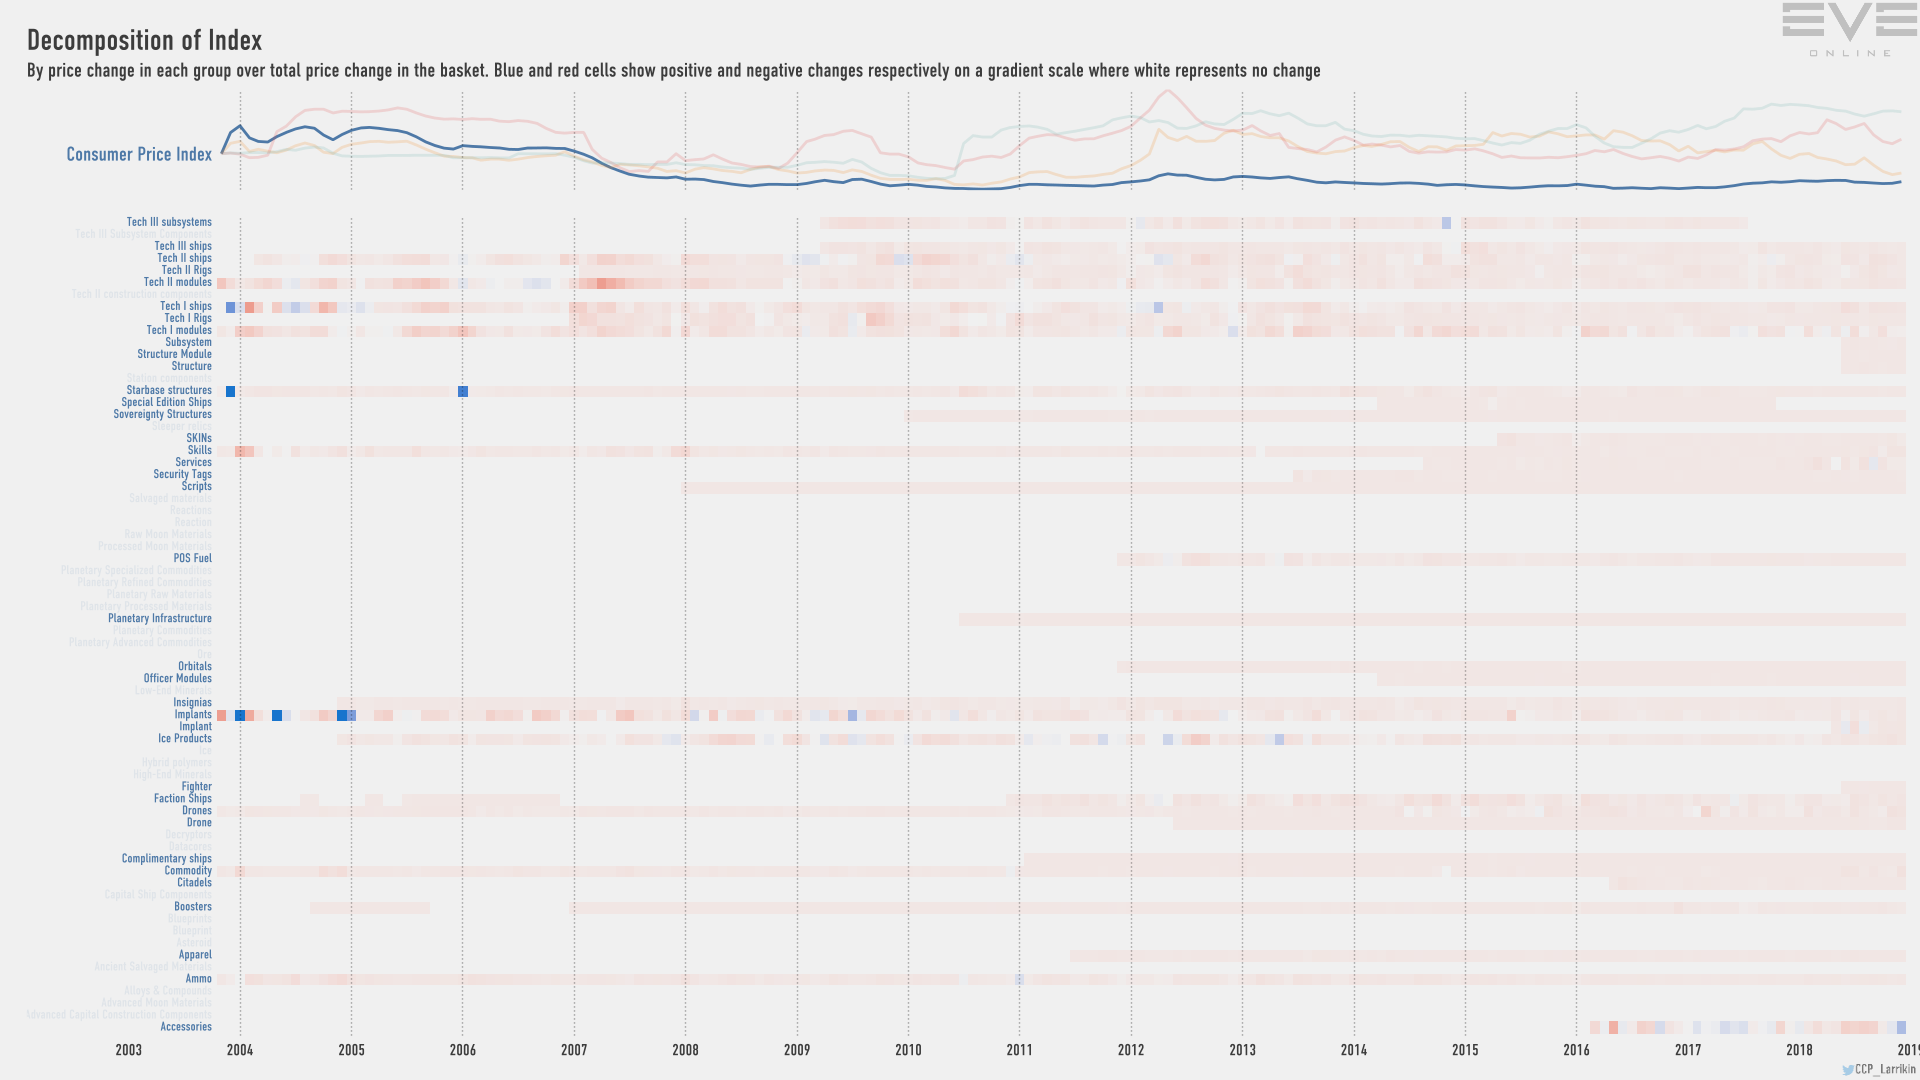
\includegraphics[width=4in]{9ea_index-decomp-ConsumerPriceIndex.png}
    \caption{The Consumer Price Index decomposition through December 2018.
    \cite{MERdec2018}}
    \label{fig:cpi}
\end{figure}

Nevertheless, in New Eden as on Earth, much economic vitality is driven by war 
and bloodshed. Producing weapons and warships is the primary economic activity
for industrial producers in EVE. The alliance with deeper pockets and more 
resources for such production is often the one that wins a war. Nevertheless,
while war is a great stimulator of New Eden's economy, it can also bring
unimaginable financial costs. 

Never in the history of EVE Online has this more evident than in the infamous
Bloodbath of B-R5RB.

\section{The bloodbath of B-R5RB}
\label{subsec:bloodbath}

In early 2014, tensions were running high in New Eden. The so-called
Halloween War, which pitted Pandemic Legion/N3 (a predecessor of the current
PanFam coalition) against CFC and a group of Russian alliances, had been 
simmering for several months. The star system of B-R5RB was under Pandemic
Legion's control, although its \textit{de jure} owners had recently changed.
In the wee hours of the morning on January 27, however, a minor hiccup proved
to be the catalyst for what still stands as the most costly battle in EVE's
history.

In null-security space, players can give ISK to CONCORD, the 
non-player-controlled police force, to establish sovereignty over a star system. 
Having sovereignty is more than a convenience: it is much more difficult to 
conquer a sovereign system than a neutral one, requiring invading forces to occupy
the space continuously for forty-eight hours without being driven away. January
27 was the renewal date for Pandemic Legion's sovereignty in B-R5RB, but ---
due to either a bug in the game or to a player's failure to ensure autopay was
enabled --- the payment was missed, and B-R5RB's sovereign status was dropped.
Ordinarily, losing sovereignty over a system is an inconvenience for an 
alliance, but not an insurmountable one; they must merely wait for a while,
make another payment, and sovereignty is restored. 

B-R5RB's importance made it different. All of Pandemic Legion's fleets massed
there for every battle. It was the location at which parts for repair and even
spare ships were stored, making the system an indispensable strategic asset. The
CFC, however, had spies in the system, and within a few hours Pandemic Legion's
bitter enemies had learned of their opportunity. Realizing their chances might
never be better, they decided to strike with everything they had. They sent
messages to pilots in their alliance with orders; soon, a massive fleet had
warped into B-R5RB. When Pandemic Legion and N3 realized this, they scrambled
every warship they had available to mount an all-out  defense. Thousands of 
ships poured into the system, and battle was joined. \cite{officialBR5RB}

\begin{figure}[ht]
    \centering
    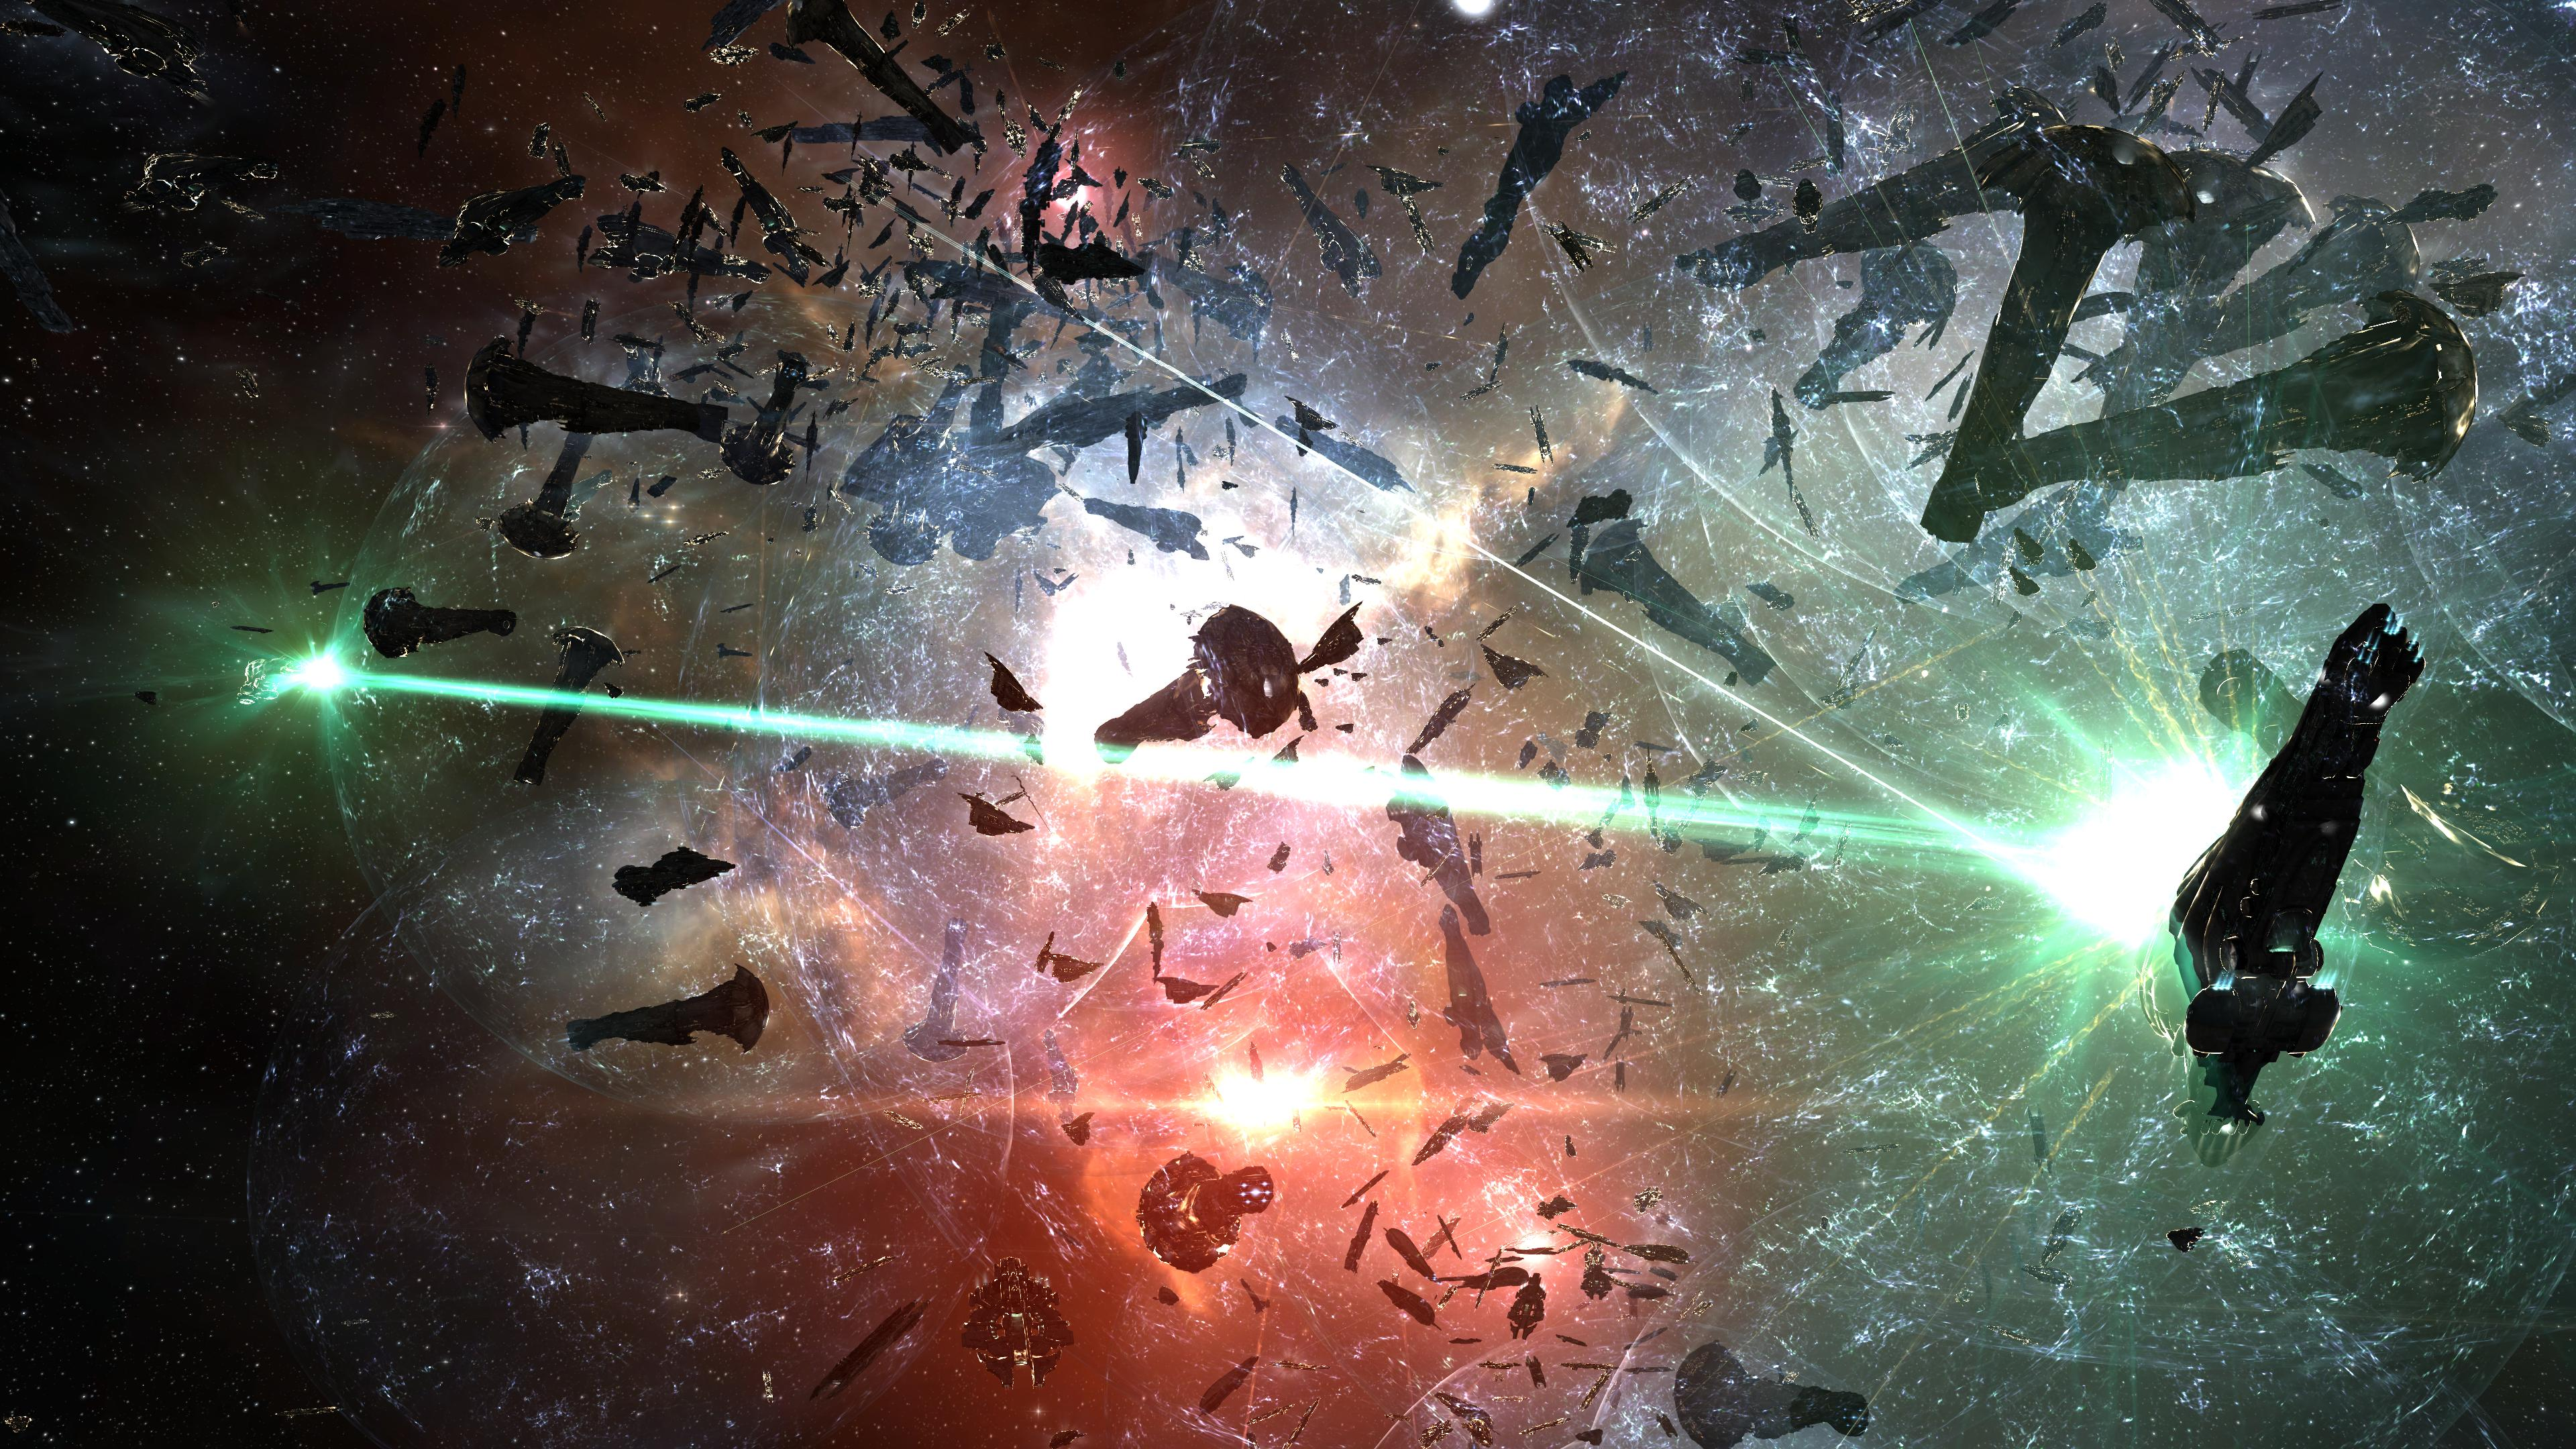
\includegraphics[width=5in]{br5rb_screenshot.jpg}
    \caption{The massive scale and seeming chaos of the battle.
    \cite{officialBR5RB}}
    \label{fig:bloodbath}
\end{figure}

Large fleet battles in New Eden feature the dreaded Titans: supercapital
warships, the largest and deadliest EVE has to offer. Each Titan costs hundreds
of billions of ISK and takes a coordinated team of hundreds of players
over a month to build. As such, only powerful alliances can construct them; 
many players never even see a Titan. Yet one can turn the tide of even a large
conflict. In addition to their massive size and bulk (the smallest Titan, called
an \textit{Avatar}, is thirteen kilometers long), each Titan can fire a
Doomsday cannon once every ten minutes, obliterating almost everything in the
path of its weapon. The size and military might of the coalitions facing one
another at B-R5RB, as well as the strategic importance of the system, meant that 
hundreds of Titans were committed to the battle.

Fighting raged for hours without either side appearing to gain an advantage, but
this changed when Pandemic Legion and N3 concentrated too much of their fire on
the Titan of the CFC fleet commander. With a herculean effort from support 
ships, this Titan took longer to destroy than its attackers expected, and other
ships were neglected to the point that the CFC and its Russian allies were able
to destroy five Pandemic Legion and N3 titans before their commander's was
lost. This discrepancy in the massive Doomsday volleys only magnified itself the
longer the fighting went on, and CFC gained an insurmountable advantage. 
Eventually, Pandemic Legion and N3 had to retreat from the system; they lost
several more Titans in this process.

By the time all EVE servers were taken offline for daily maintenance, the 
bloodbath had gone on for 21 hours. More than 7,500 players participated.
Seventy-five Titans were destroyed (59 belonging to Pandemic Legion and N3), 
more than were even seen in most battles. Thousands of smaller ships were also
destroyed. The total economic losses to both sides totaled over 
11,000,000,000,000 ISK. By reference to PLEX, a \$15/month in-game
subscription which is also available to purchase on in-game markets, it has
been estimated that the battle cost the equivalent of \$300,000 of in-game
ships, weapons, and cybernetic implants. 

The sheer scale of B-R5RB demonstrates not only the depth and complexity of
EVE Online, but also the dedication and intensity of its players. Player-vs.-
player combat is the heart and soul of EVE, and its magic comes from the 
capsuleers who make it possible. In this work, we seek to understand a small
piece of this magic.


\section{Outline}
\label{subsec:outline}

In \cref{sec:data}, we discuss the objectives of the project, the data on which
our analyses are based, and how they were processed into a form suitable for
statistical modeling. \cref{sec:stats} contains a discussion of the statistical
analysis performed after the data were processed, including the final model found. 
Finally, in \cref{sec:disc}, we explore the conclusions which we can draw from
the model and present directions whereby continuing research could improve it.

\clearpage
\chapter{Data collection and processing}
\label{sec:data}

Our project began with a request for economic analysis from a veteran EVE
player. Initially, our client's guidance was vague; it was thought that we could
analyze data leading to an overall picture of economic health in EVE, perhaps as
relating to the real world. However, the incredible amount and complexity of
economic data available in-game (and the even-more-complex nature of real-world
financial data) soon convinced us to narrow our scope. We would analyze 
economic aspects of one small, but major part of EVE's universe:
player-vs.-player combat.

The first crucial aspect of the analysis was to find these data; fortunately,
EVE makes them incredibly easy to obtain.

\section{The Monthly Economic Report}

CCP Games, the developers of EVE Online, regularly release a collection of files
called the Monthly Economic Report (MER) on EVE's official website.
\cite{MERdec2018}
These reports contain a wealth of detailed economic data collected in the game: 
from consumer and producer price indices, to the velocity of ISK over the past 
month, to traffic reports charting the regions with the most stargate jumps over
the course of the month (\cref{fig:jumps}).

\begin{myfigure}[blanker]
    \centering
    \captionsetup{type=figure}
    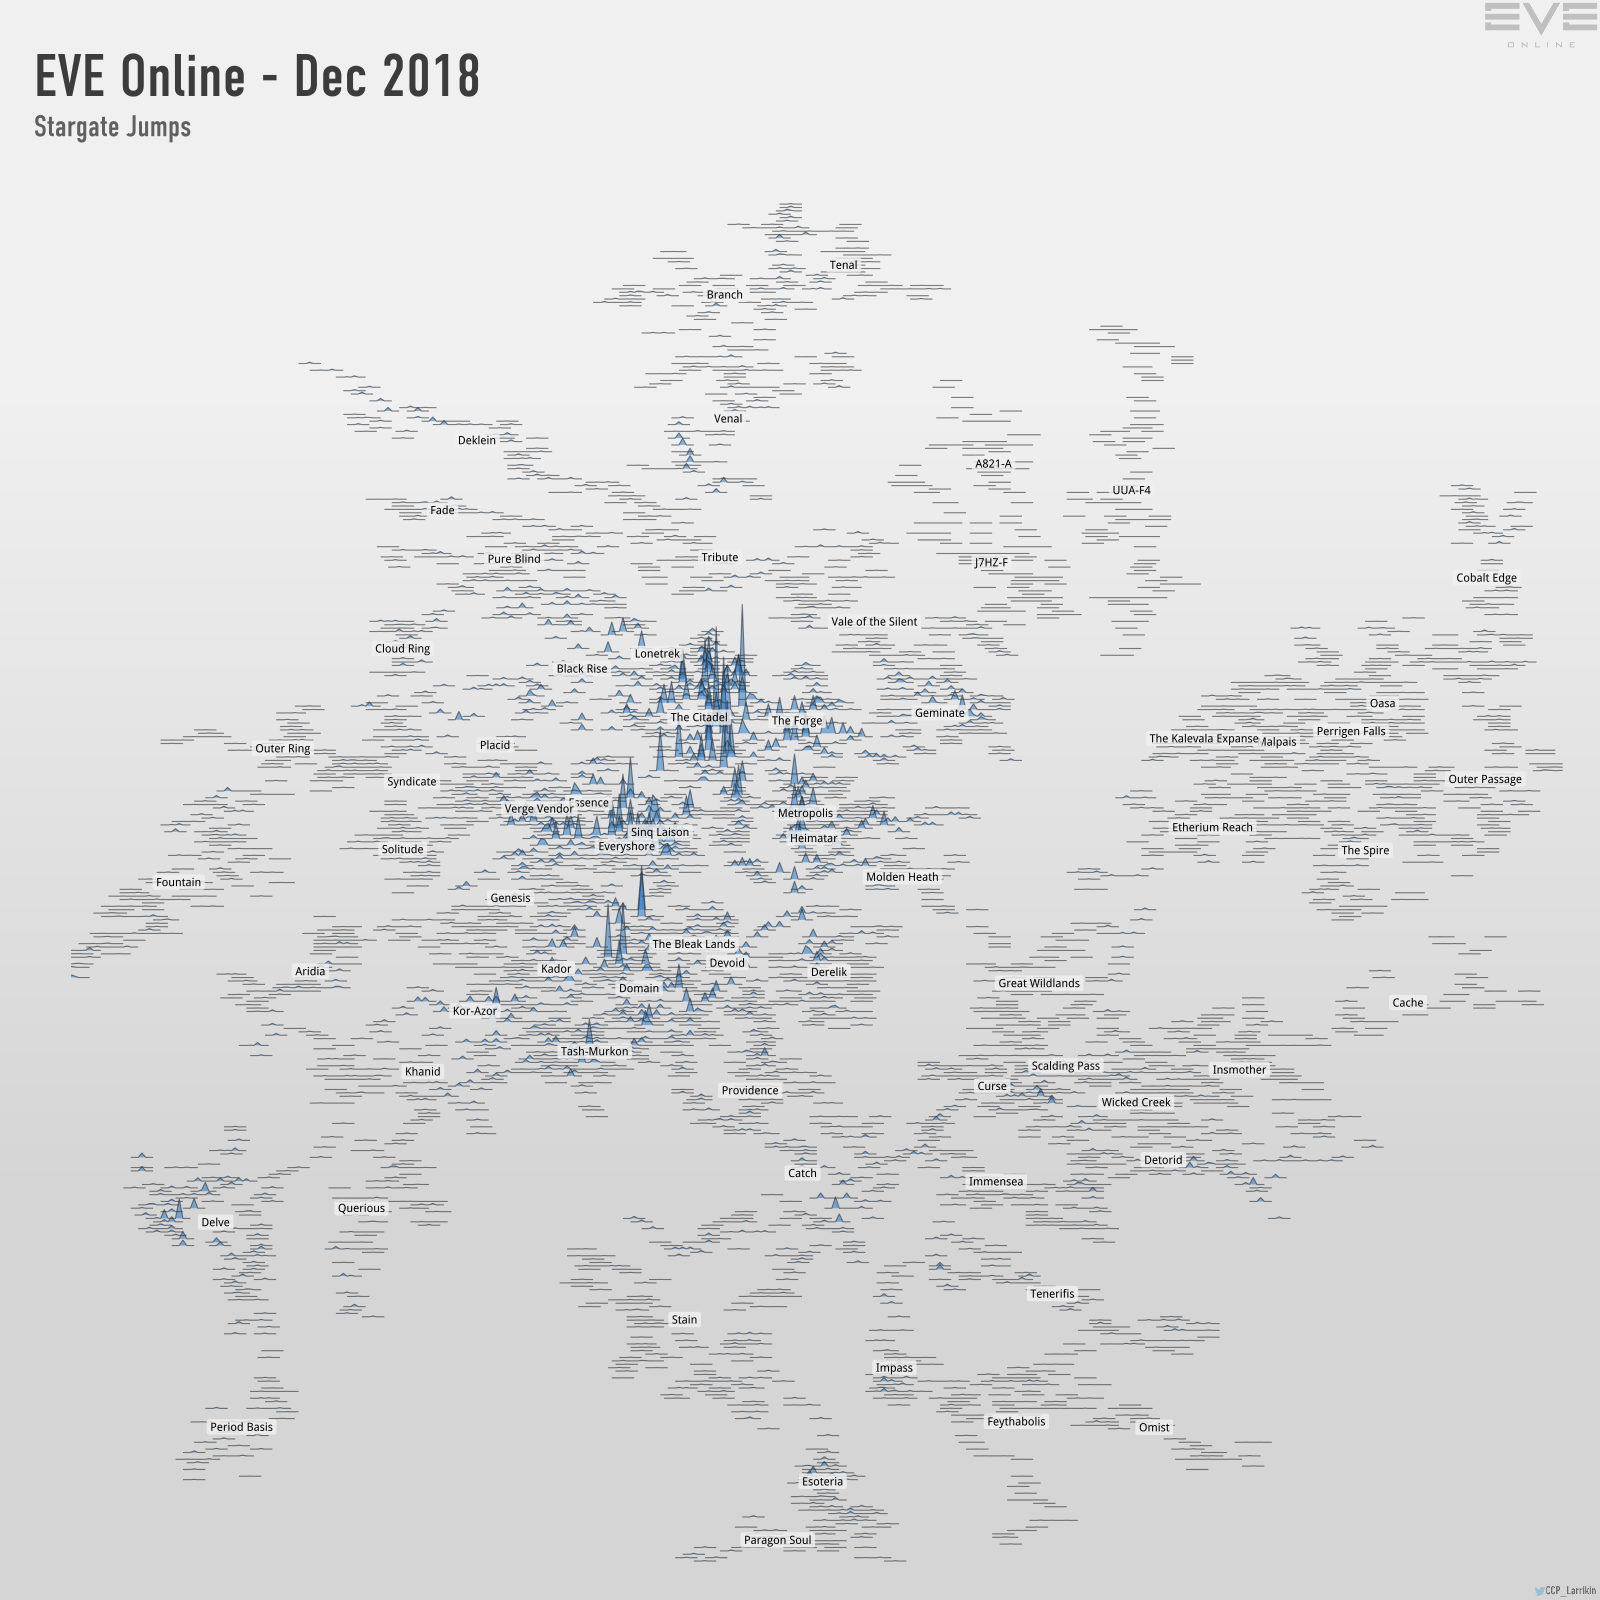
\includegraphics[height=\myspace]{stargate_jumps.png}
    \captionof{figure}{The stargate jumps for December 2018.\cite{MERdec2018}}
    \label{fig:jumps}
\end{myfigure}

In this work, we are interested in the economics of salvage and recovery in the
aftermath of a ship battle. In particular, we wish to predict the ISK that will
be recoverable once a ship is destroyed, whether by the destroyer or by the
allies of the victim. We must determine all the predictions directly from the
MER data; we do not possess expert knowledge that would allow us to make
\textit{a priori} hypotheses.

\section{The killdump}

Our data come from just one file included in each MER: {\ttfamily Killdump.csv}.
This file, typically around 60 megabytes in size, logs in plain text data about
every starship destroyed in New Eden over the course of the preceding month. The
information included about the destroyed ship and the circumstances surrounding 
its destruction is substantial:
\begin{enumerate}[nolistsep,label=\textbf{--}]
    \item The affiliations of both the destroyed ship's player and the 
    destroyer, at the corporation and alliance levels;
    \item The specific and general type of ship destroyed;
    \item The date and time of destruction, to the nearest second;
    \item The solar system and region in which the ship was destroyed;
    \item The ISK lost by the destroyed ship's player;
    \item The ISK destroyed irrevocably; and
    \item The bounty claimed by the destroyer, if any.
\end{enumerate}

The killdump contains a convenient way to represent the ISK recoverable after
the destruction of a starship. Noting that the ISK lost is always at least as
large as the ISK destroyed in a destruction log, we defined ISK recoverable by
\begin{align} \label{eq:response}
    \textrm{ISK recoverable} &= \textrm{ISK lost} - \textrm{ISK destroyed}.
\end{align}


We analyzed the killdumps from October through December 2018, for a total of
three months of data. Each month, about 375,000 starships were destroyed in
New Eden, which meant that we were faced with the task of analyzing over one
million data points. On a typical home computer, this is far too much data to
quickly and reliably analyze; it quickly became apparent that some reduction
in the sheer amount of data was necessary.

\section{Pruning the data}
To this end, we turned to the Python programming language \cite{python} for its
ease of use for file management. We found, first, that approximately one third 
of all ships destroyed were Capsules: escape pods for players' avatars that are
automatically ejected when the their ships are destroyed. Capsules can be
destroyed independently of the ships from which they come, but there is never 
any ISK recoverable from the destruction of a capsule. As such, we purged each
entry whose ship group was a capsule, removing it from the analysis.

We also found that the killdump contained too much information about each ship
destroyed. There are tens of thousands of corporations in New Eden; recording
the corporate affiliation of the victim and the killer affords a level of
specificity that would make any statistical model impossible to interpret.
Furthermore, it would present a great danger of \textit{overfitting}: finding
patterns  in the data by chance that do not carry over to months outside the
three we considered. Analogously, the 7,500-plus star systems are too specific 
to analyze. Thus, we removed these variables from our cleaned dataset.

At this point, we had reduced our data to 813,533 data points, each with 13
different variables stored. We were at a point at which we could begin the
so-called exploratory data analysis, searching for patterns and planning
initial models, but we would still need to reduce the number of data points
substantially before we were ready for a final model. This exploration, however,
called for a different tool.

\section{Exploratory data analysis}

That tool, the standard for statisticians the world over, is R. 
\cite{R} When paired with a collection of packages known as the Tidyverse,
\cite{tidyverse} R allows powerful data processing, statistical exploration,
analysis, and visualization to be performed relatively intuitively, often with
minimal effort. All analysis and modeling were performed in R, version 3.5.3, 
and all plots (except the autocorrelation plot below) were generated using the
\texttt{ggplot2} package. \cite{ggplot2}

Since we still had over 800,000 data points, we found it necessary to condense
the data further and to summarize across unneeded variables. First, we discarded
date-time information except for the hour of day at which the ship's destruction
occurred. Since our analysis strategy did not involve time-series 
considerations, we did not keep track of whether some ship was destroyed before 
another. 

Initial exploration revealed that, although alliances are a larger social unit 
than are corporations in EVE, there were still too many alliances to interpret
a model incorporating them, and overfitting was still a danger. As such, we 
condensed our data across the alliances, considering only the average ISK
recoverable from each.

Our analysis of the hour of day at which the ship destruction occurred revealed
that time is not an effective way to predict the ISK recoverable from a
destroyed starship. However, we did discover an interesting recurrence, gleaned
from the autocorrelation function (\cref{fig:acf}). There is a spike at about
24 hours of lag, indicating that there is a relationship between ships 
destroyed at the same time each day. Furthermore, the autocorrelation takes about
5 hours to decay below the blue threshold. This indicates a pattern in player
activities: the typical session in New Eden lasts up to about five hours, and
players tend to log on at approximately the same time each day. We did not,
however, explore this relationship more carefully, because of the weak 
relationship between ISK recoverable and the time.

\begin{figure}[ht]
    \centering
    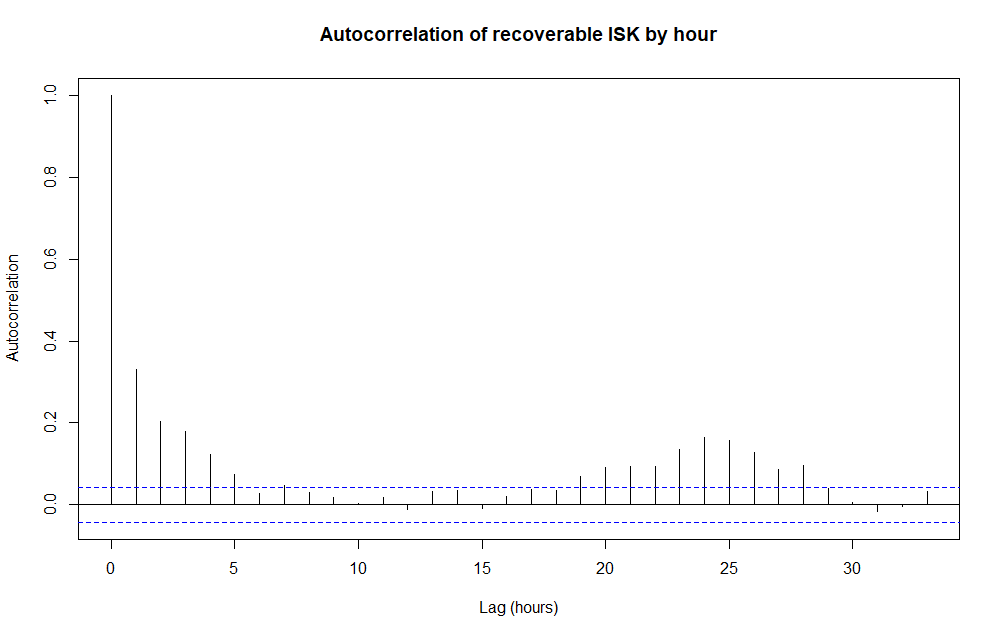
\includegraphics[width=4in]{ACF_byHour.png}
    \caption{The recurrence in time.}
    \label{fig:acf}
\end{figure}

Even after removing the specific name of each ship class, there remained 89
different groups of ships, still too many for an effective analysis. As such,
we grouped these variables still more tightly, into 11 different kinds. We
delineated between ships designed for combat and for noncombat roles, and 
recorded in broad strokes the size of the ship. \cref{tab:shipkinds} shows
the final kinds we chose. Freighters are a special class of noncombat ship;
they tend to carry very valuable cargo and hence have a large amount of ISK
recoverable from their wreckage. Finally, starbases are owned by players but
are not mobile; thus, they are not easily placed into combat and noncombat 
categories. Their ISK recoverable varies widely.

\begin{table}[ht]
    \centering
    \begin{tabular}{@{}lll@{}}
        \toprule
        Size & Combat representative & Noncombat representative \\
        \midrule
        Small & Frigate & Expedition frigate \\
        Medium & Cruiser & Blockade runner \\
        Large & Battleship & Industrial command ship \\
        Capital & Dreadnought & Industrial capital ship \\
        Supercapital & Titan & N/A \\
        \midrule
        \multicolumn{2}{l}{\textbf{Additional ship kinds:}} & Representative \\
        \midrule
        \multicolumn{2}{l}{Freighter} & Jump freighter \\
        \multicolumn{2}{l}{Starbase} & Control tower \\
        \bottomrule
    \end{tabular}
    \caption{The final ship kinds.}
    \label{tab:shipkinds}
\end{table}

\clearpage
\chapter{Modeling the ISK recoverable}
\label{sec:stats}

This processing reduced the size of our dataset to a mere 150,008 entries, and the
number of fields for each entry from 17 to 8. While still substantial, this amounted
to about one tenth of the initial number of ships we had to consider. From here, we
were ready to perform our statistical analyses.

Creating exploratory models and hunting for patterns, we found that there are three
useful predictors of ISK recoverable: 
\begin{enumerate}[nolistsep,label=(\arabic*)]
    \item The kind of ship that was destroyed;
    \item The region of New Eden in which the ship was destroyed;
    \item The amount of bounty placed on the destroyed ship.
\end{enumerate}

Armed with this knowledge, we could seek for a final, predictive model. In
statistical language, we place a hat on a variable which we intend to predict. As
such, our research question translated into the framework of statistical modeling is
as follows:

\begin{align} \label{eq:general}
    f(\widehat{R}) &= g(\textrm{ship kind},\textrm{region},\textrm{bounty}),
\end{align}

where
\begin{enumerate}[nolistsep,label=\textbf{--}]
    \item $\widehat{R}$ is the predicted ISK recoverable from any destroyed
    starship, and
    \item $f,g$ are some mathematical functions.
\end{enumerate}

Our modeling task became to determine the identity of $f$ and $g$. An important
consideration was \textit{parsimony}; that is, we prefer simpler models that can
be explained as well as used for prediction. There were enough data entries in 
the killdump before our reduction and processing that we could likely have created
a model under the machine learning paradigm; in this framework, we care only about
predictive power and do not even attempt to understand why the model parameters 
take the forms they do. For increased usefulness and memorability to players, 
however, we prefer interpretability, so we use a classical and parsimonious model.

Our first consideration, then, was how to determine $f$.

\section{Transforming the response}

Much of the validity of statistical models hinges on the normality of the response:
if we were to sample the quantity we wish to measure infinitely many times, standard
models assume that the distribution of these samples should follow the classical
normal bell curve. Unfortunately, the ISK recoverable are not normally distributed.

\begin{figure}[ht]
    \centering
    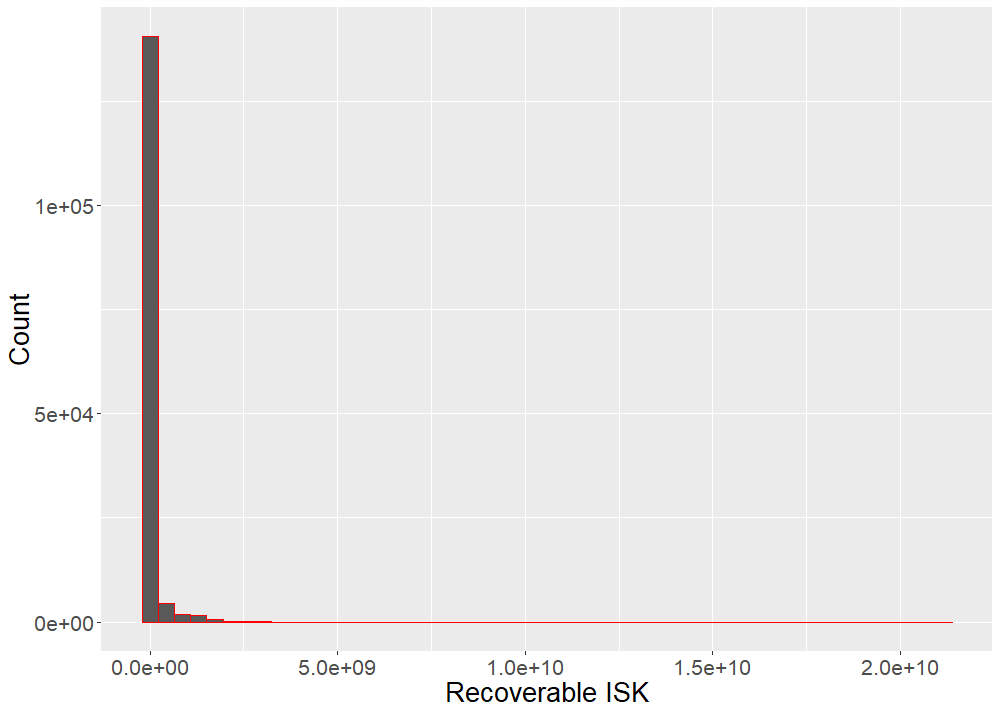
\includegraphics[width=4.5in]{Hist_ISKRecoverable.png}
    \caption{The distribution of ISK recoverable.}
    \label{fig:hist}
\end{figure}

The pattern seen in the histogram of \cref{fig:hist} --- a sharp decline in the
number of ships observed with each increase of ISK recoverable --- is actually
retained if we focus more closely on the tail of the histogram. This property is
called \textit{memorylessness}, and is characteristic of the exponential 
distribution. While an exponentially distributed response variable cannot be
analyzed with a standard linear model, it is fortunately fairly easy to normalize
by a logarithmic mathematical transformation. Attempting this, we chose a logarithm
in base 10 for ease of interpretation and prepared another histogram.

\begin{figure}[ht]
    \centering
    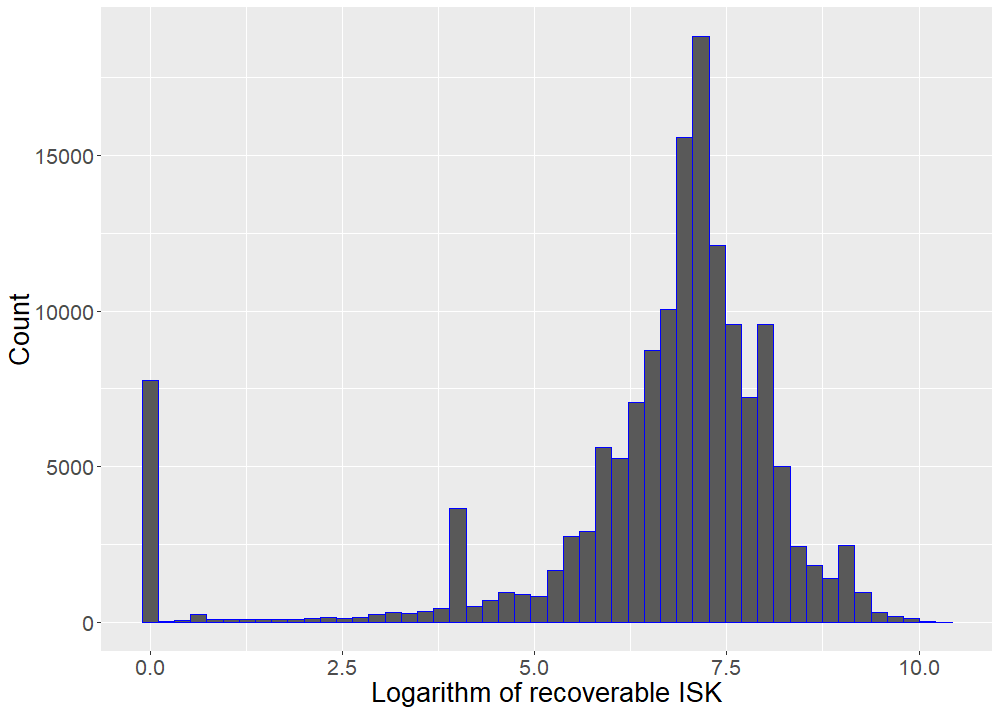
\includegraphics[width=4.5in]{Hist_LogRecoverable.png}
    \caption{The base-10 logarithm of ISK recoverable.}
    \label{fig:loghist}
\end{figure}

\cref{fig:loghist}, the histogram after the logarithmic transform, shows much
better agreement with the bell curve we expect and hope for. There is a spike at
zero $\log{(\textrm{ISK recoverable})}$, which is a cause for minor concern, but
because of the sheer quantity of our data we should still have enough predictive
power to find what we are looking for.

The meaning of the exponential distribution of the ISK recoverable means that, at
least in this context, the economics of New Eden are concerned with \textit{orders
of magnitude} instead of with untransformed numbers. Instead of talking about a
ship five times more valuable than another, we would discuss a ship $10^5 = 
100,000$ times more valuable. In addition, the peak at approximately 7.3 indicates
that the mean expected ISK recoverable is about $10^{7.3} = 19,950,000$ ISK.

Thus far, then, we have determined that $f(\widehat{R}) = \log_{10}{\widehat{R}}$, 
so it remains for us to determine $g$, the function specifying how the predictor
variables influence the expected ISK recoverable:

\begin{align} \label{eq:loggedResp}
    \log_{10}{\widehat{R}} &= g(\textrm{ship kind},\textrm{region},\textrm{bounty}).
\end{align}

\section{The predictors}

We needed to consider similar distributional modifications in the predictors, if
such were found to be appropriate, as well as \textit{interactions} between them:
whether the effect of one predictor on the ISK recoverable changes depending on 
the value of another predictor. Additionally, both the ship kind and the region
in which the ship was destroyed are \textit{categorical} predictors, with discrete,
defined levels: it is (for instance) impossible for a single ship to be part 
cruiser and part frigate, while any amount of bounty is in principle possible. This
limits the form of the mathematical functions that can describe them, but 
interpreting coefficients for a discrete predictor is relatively simple.

\subsection{Ship kind}

As could perhaps be expected, the kind of ship destroyed is the strongest 
predictor of ISK recoverable: destroying a behemoth Titan or other supercapital
ship will provide a far more valuable salvage than will eliminating a 
comparatively tiny corvette. \cref{fig:shipkinds} displays all eleven ship kinds
we considered as a boxplot: the central line for each ship kind shows the median
observed ISK recoverable (on a logarithmic scale), while the upper and lower 
extremes of the box show the third and first quartiles respectively. The dots
outside the box are more extreme values.

\begin{figure}[ht]
    \centering
    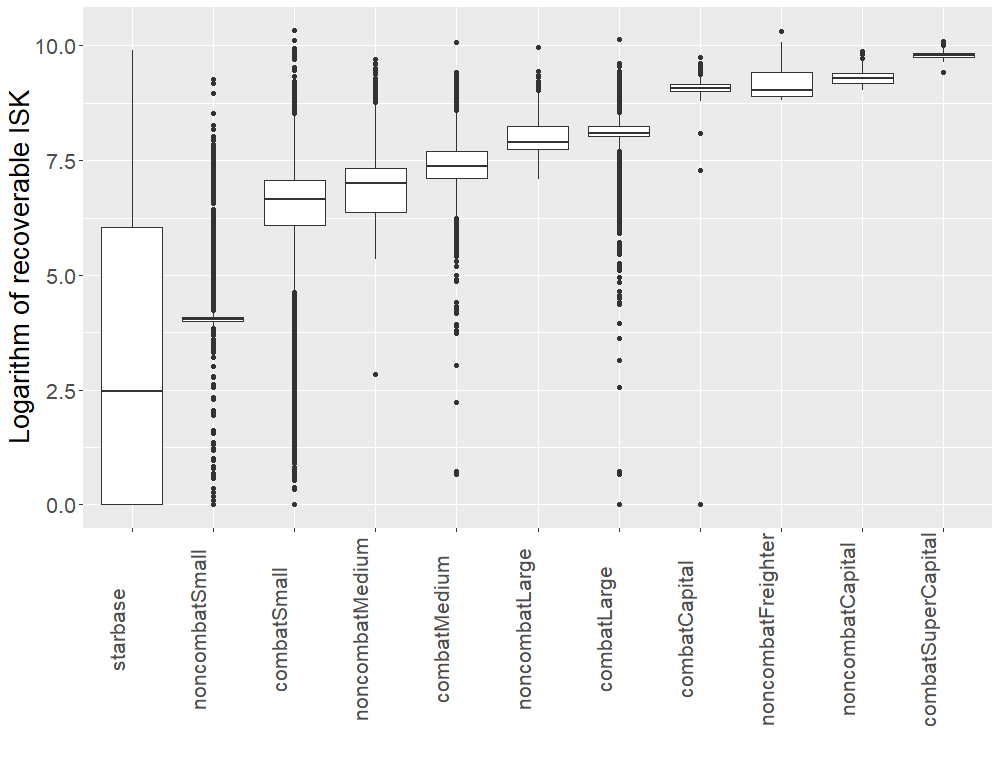
\includegraphics[width=4.5in]{Boxplot_ShipKind.png}
    \caption{The ship kinds ordered by ISK recoverable.}
    \label{fig:shipkinds}
\end{figure}

Evidently, we observe a large degree of variability in the ISK recoverable for 
smaller ships, but the pattern grows tighter for the larger ones. We do observe
a very noticeable distinction between most of the ship types. In most cases, the 
entire box is vertically separated from all but its closest neighbors. Often, the
median ISK recoverable from one ship to another differs by close to a full unit
on the logarithmic scale, meaning that the one returns nearly ten times the ISK
recoverable as the other.

Despite its undeniable utility as a predictor, the ship kind has an important
limitation. Most players do not have the ability to take on a Titan in combat
for profit. Even a group of dozens of players with formidable battleships would be
unlikely to destroy a lone Titan, whose nigh-impenetrable armor and shields would
keep it alive while its awful Doomsday cannon wreaked havoc on its would-be
assailants. On the other hand, destroying a corvette with a Titan might not
provide enough recoverable ISK to cover the cost of the ammunition it took to
destroy the smaller craft. Thus, the kind of ship an enterprising pirate or bounty
hunter is able to destroy is determined largely by the kind of ship he or she can
afford to pilot. In other words, this predictor is useful for narrowing the range
of expected ISK that can be recovered from a destroyed ship, but not for deciding
what kind of ship to attack to maximize profit. For that, the other two predictors
must be considered.

\subsection{Region}

There are 102 regions in EVE; each has its own predicted value for the logarithm of
ISK recoverable. This is far too many to place on a boxplot like the ship kind.
Instead, in \cref{fig:regions}, we highlight a few regions found to be the most
lucrative. There is not an easily interpretable pattern: for instance, Period
Basis, in the southwest corner of the map, is a dead-end region with nothing 
beyond it, while Scalding Pass, in the east, is a major thoroughfare. These two
regions are in null-security space, while Black Rise and the Bleak Lands, nearer 
the map's center, are in high-security space, heavily patrolled by the in-game
policing force CONCORD. As such, interpreting the reasons why these regions give
larger predictions for recoverable ISK than do their neighbors requires knowledge
that we do not possess; we might be able to obtain it by consulting with a
well-traveled and expert player.

\begin{figure}[ht]
    \centering
    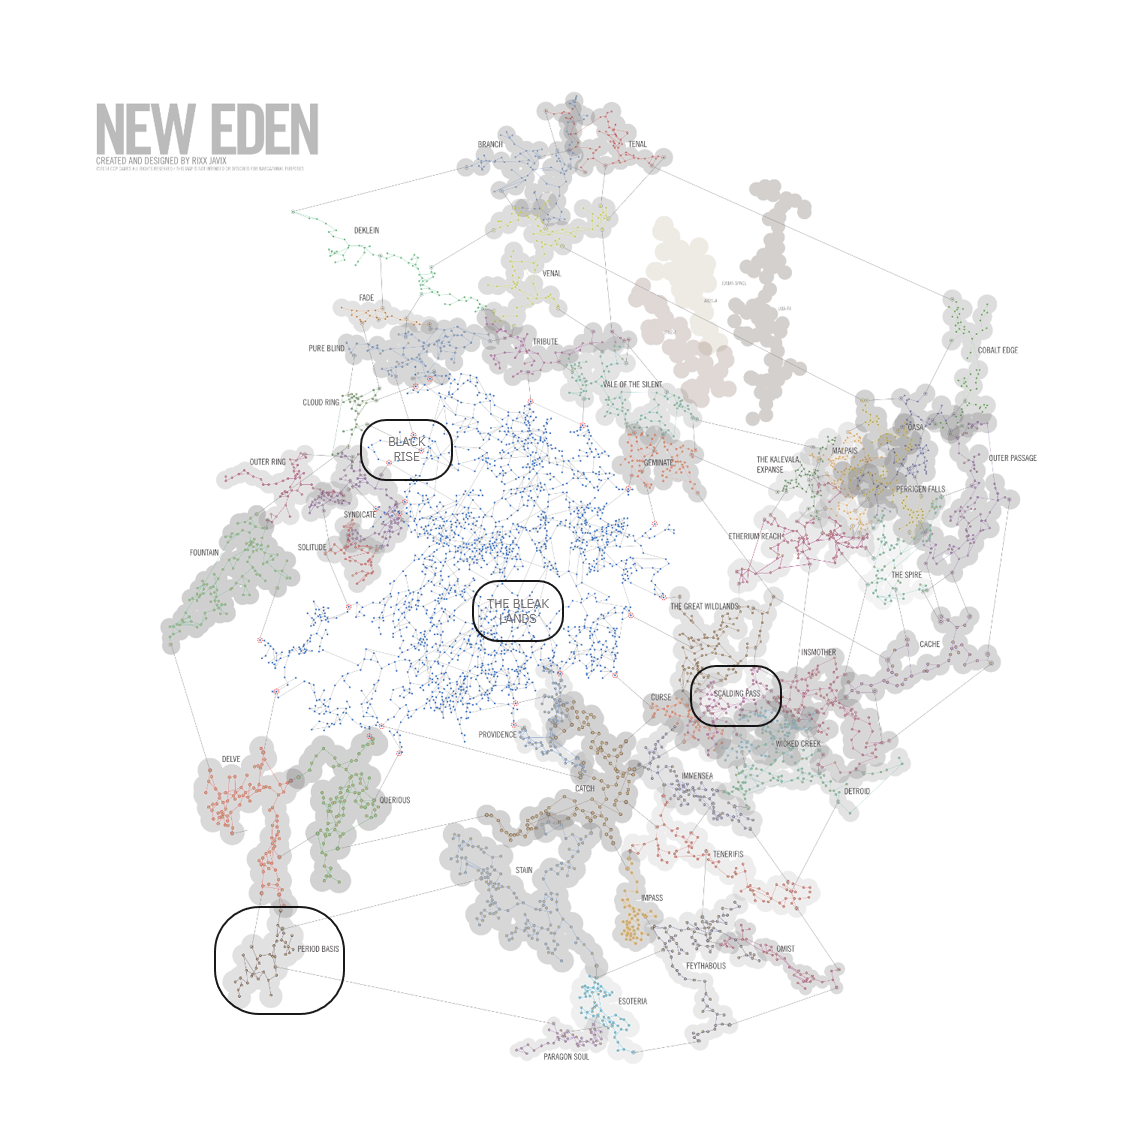
\includegraphics[width=4.5in]{valuableRegions.png}
    \caption{Some valuable regions in Known Space.}
    \label{fig:regions}
\end{figure}

Of note, however, is that the most valuable regions do not appear on this
or any other map of New Eden. The map can display only Known Space regions, which
have a permanent network of stargates linking them; players can at their 
convenience warp through these stargates to travel nearly instantaneously between
regions separated by large swathes of empty space. Some regions --- such as H-R00032,
the most lucrative region for ISK recoverable in New Eden --- are in Wormhole
Space, and have no such travel network. Instead of set stargates, Wormhole Space
can be reached only by the eponymous wormholes, which appear and disappear
unpredictably in random locations of Known Space. Capsuleers who venture into
Wormhole Space do not know where or when they will be able to return, so they must
prepare accordingly. Thus, targets in Wormhole Space are more heavily loaded with
supplies and weapons, making them more valuable targets for salvage if destroyed.
However, this heightened preparedness makes Wormhole Space a more dangerous field, 
for pirates and potential victims alike.

\subsection{Bounty}

We found that bounty, our only continuous predictor, was exponentially distributed
much like the ISK recoverable, so we applied the same logarithmic transformation
(in base 10) to it as we did the other. This provides additional evidence toward
economics in EVE being centered around orders of magnitude.

In general, we found that an increase in the bounty placed on a ship predicts an
increased ISK recoverable when it is destroyed; both values are interpreted on a
logarithmic scale. The cluster of data points along the bottom edge of
\cref{fig:bounty} indicate that this increase is actually independent of the ISK
directly gained by cashing in the bounty; it may be that wanted criminals need to
carry more valuable items with them because it is more difficult for them to dock
at most markets to resupply.

\begin{figure}[ht]
    \centering
    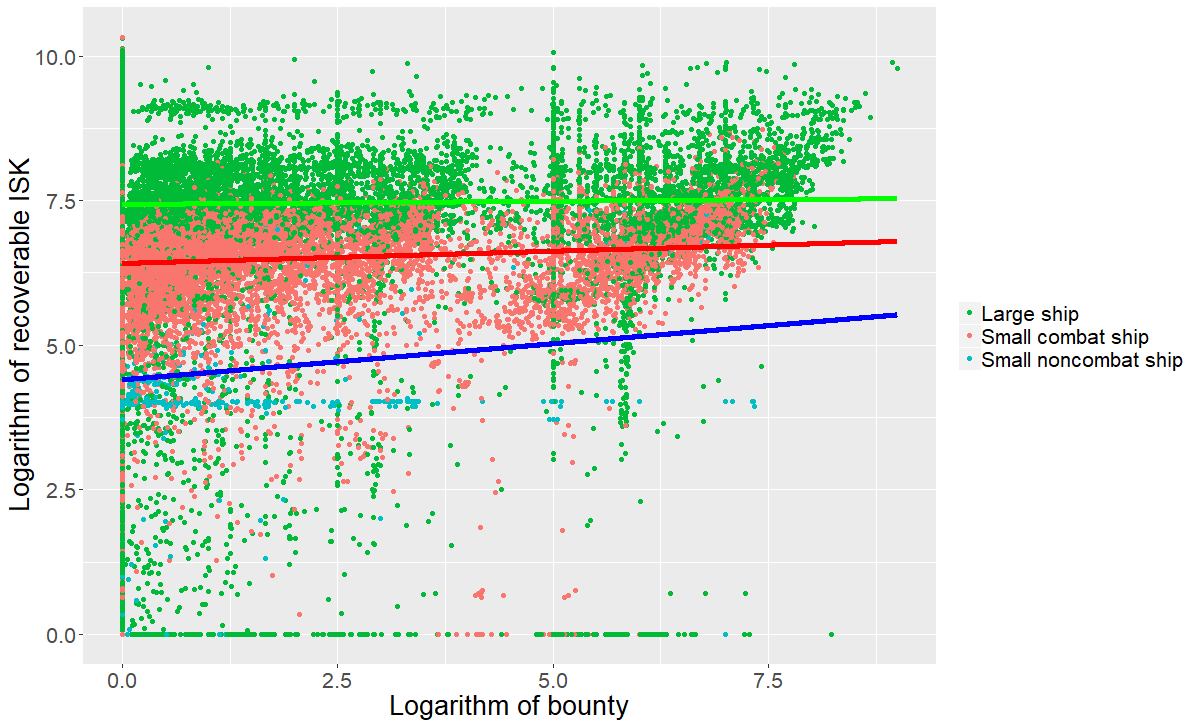
\includegraphics[width=4.5in]{bountyPredPlot_legend.png}
    \caption{The predicted changes in ISK recoverable based on bounty.}
    \label{fig:bounty}
\end{figure}

Most ships share the same predicted slope, seen in green in the figure. However,
smaller ships have a more pronounced effect of bounty. Small noncombat ships such
as mining frigates, seen in blue, have their ISK recoverable value most strongly
influenced by the bounty. In between are small combat ships such as frigates and 
destroyers (red). 

Thus, we find that it is better to choose a ship to destroy with a larger bounty
in all cases, but that the bounty is more important to focus on when the target
is a smaller ship. However, it is likely the case that competition from other 
bounty hunters is stiffer for criminals with a larger bounty; players must weigh
their selection of values for this predictor carefully as well when attempting to
destroy another ship for profit.

\section{The final model}

Having interpreted each predictor, we were ready for a final, quantitative model,
seen in \cref{eq:final}:

\begin{align} \label{eq:final}
    \log_{10}{\widehat{R}} &= \mu + \sigma_i + \rho_j + (\beta_0 + 
    \beta_{sc} x_{sc} + \beta_{sn} x_{sn}) \log_{10}{b}, 
\end{align}

where
\begin{enumerate}[nolistsep,label=\textbf{--}]
    \item $\widehat{R}$ is the predicted ISK recoverable (we add 1 to the value 
    before taking the logarithm to remove negative numbers from the transformed
    value);
    \item $\mu$ is the baseline prediction, for the least valuable ship kind
    (starbases), the least lucrative region (the Great Wildlands), and a bounty
    of zero (on the log scale);
    \item $\sigma_i$ is the adjustment made based on the ship kind --- there are
    ten values that $\sigma$ can take;
    \item $\rho_j$ is the adjustment made based on the region, with 101 additional
    values possible;
    \item $\beta_0$ is the baseline slope of ISK recoverable based on the logarithm
    of bounty, which has value $b$ (again, add 1 to $b$ before taking the logarithm
    to prevent errors for ships with zero bounty);
    \item $\beta_{sc}$ is the change in slope for small combat ships, which are
    indicated by $x_{sc}$; and
    \item $\beta_{nc}$ is the change in slope for small noncombat ships, indicated 
    by $x_{nc}$.
\end{enumerate}

We list the various coefficients below. \cref{tab:coeffs} shows most of them;
however, since there are so many regions, their corresponding coefficients 
$\rho_j$ are placed in a separate table, \cref{tab:regions}. Recall that the
value of each $\rho_j$ refers to the change in the base-10 logarithm of the
predicted ISK recoverable for a ship destroyed in that region, compared to
the predicted logarithm of ISK recoverable for a ship destroyed in the 
baseline region of the Great Wildlands. The regions' coefficients are not
influenced by different ship kinds or the bounty on the starship.

\begin{table}[ht]
    \centering
    \begin{tabular}{@{}lll@{}}
        \toprule
        Coefficient & Interpretation & Value \\
        \midrule
        $\mu$ & Baseline ISK recoverable & 2.619576 \\
        $\beta_0$ & Larger ships' bounty effect & 0.011031 \\
        $\beta_{sc}$ & Small combat bounty change & 0.031243 \\
        $\beta_{nc}$ & Small noncombat bounty change & 0.113815 \\
        \midrule
        $\sigma_i$: & Small noncombat ships & 1.398508 \\
         & Small combat ships & 3.410008 \\
         & Medium noncombat ships & 3.923020 \\
         & Medium combat ships & 4.430100 \\
         & Large noncombat ships & 4.954883 \\
         & Large combat ships & 5.073813 \\
         & Capital combat ships & 6.075118 \\
         & Freighters & 6.194115 \\
         & Capital noncombat ships & 6.291156 \\
         & Supercapital combat ships & 6.837297 \\
        \bottomrule
    \end{tabular}
    \caption{The model coefficients (except for $\rho_j$).}
    \label{tab:coeffs}
\end{table}

\begin{center}
\begin{longtable}{lllll}
    \toprule
    Region & Value & \hspace{1em} & Region & Value \\
    \midrule
    \endfirsthead
    
    \midrule
    \multicolumn{5}{r}{(Continued on next page)} \\
    \bottomrule
    \endfoot
    
    \bottomrule
    \\[-4pt]
    \caption{The coefficients $\rho_j$ for region.}
    \label{tab:regions}
    \endlastfoot
    
    \toprule
    Region & Value & \hspace{1.5em} & Region & Value \\
    \midrule
    \endhead
    
    Syndicate               & 0.029415 & & Curse            & 0.105452 \\
    Tribute                 & 0.216711 & & Venal            & 0.200904 \\
    Oasa                    & 0.081728 & & Cloud Ring       & 0.253100 \\
    Vale of the Silent      & 0.230389 & & Outer Passage    & 0.150636 \\
    Etherium Reach          & 0.185224 & & A-R00001         & 0.443430 \\
    The Kalevala Expanse    & 0.205190 & & Outer Ring       & 0.225972 \\
    Cache                   & 0.590705 & & The Spire        & 0.201942 \\
    A-R00002                & 0.345095 & & Genesis          & 0.327192 \\
    Tash-Murkon             & 0.353134 & & Feythabolis      & 0.370441 \\
    Perrigen Falls          & 0.095338 & & Kador            & 0.592372 \\
    Pure Blind              & 0.232976 & & Derelik          & 0.157844 \\
    K-R00033                & 0.161684 & & Cobalt Edge      & 0.217216 \\
    Khanid                  & 0.361856 & & B-R00008         & 0.433706 \\
    H-R00032                & 0.816952 & & Sinq Laison      & 0.207575 \\
    Lonetrek                & 0.207134 & & C-R00010         & 0.654473 \\
    Everyshore              & 0.450422 & & A-R00003         & 0.444546 \\
    B-R00006                & 0.531530 & & Kor-Azor         & 0.242345 \\
    Paragon Soul            & 0.347293 & & The Forge        & 0.302484 \\
    Querious                & 0.461567 & & Geminate         & 0.334999 \\
    C-R00011                & 0.634491 & & Malpais          & 0.264273 \\
    C-R00012                & 0.520463 & & C-R00013         & 0.671173 \\
    Verge Vendor            & 0.300227 & & Solitude         & 0.217974 \\
    Metropolis              & 0.276126 & & Tenerifis        & 0.520070 \\
    Fountain                & 0.514110 & & Impass           & 0.441969 \\
    B-R00005                & 0.547217 & & Catch            & 0.402157 \\
    Deklein                 & 0.388507 & & Molden Heath     & 0.353258 \\
    Essence                 & 0.290248 & & Wicked Creak     & 0.406289 \\
    Stain                   & 0.473259 & & Domain           & 0.362200 \\
    Heimatar                & 0.322869 & & Tenal            & 0.517601 \\
    B-R00004                & 0.511074 & & Fade             & 0.531845 \\
    Delve                   & 0.444058 & & C-R00015         & 0.697176 \\
    Devoid                  & 0.346900 & & Insmother        & 0.537153 \\
    Placid                  & 0.291159 & & The Citadel      & 0.384610 \\
    Aridia                  & 0.366785 & & E-R00027         & 0.604972 \\
    E-R00028                & 0.483441 & & Esoteria         & 0.531096 \\
    Branch                  & 0.525390 & & Providence       & 0.512561 \\
    Immensea                & 0.533066 & & Omist            & 0.694132 \\
    Detorid                 & 0.439598 & & E-R00026         & 0.721486 \\
    C-R00014                & 0.675879 & & C-R00009         & 0.780562 \\
    E-R00029                & 0.656755 & & D-R00021         & 0.538862 \\
    E-R00024                & 0.640956 & & Black Rise       & 0.432332 \\
    Period Basis            & 0.613525 & & D-R00022         & 0.508852 \\
    F-R00030                & 0.779741 & & D-R00023         & 0.555466 \\
    The Bleak Lands         & 0.384371 & & D-R00017         & 0.629396 \\
    Scalding Pass           & 0.573571 & & D-R00019         & 0.567772 \\
    D-R00018                & 0.627241 & & D-R00016         & 0.743277 \\
    E-R00025                & 0.658958 & & B-R00007         & 0.508703 \\
    G-R00031                & 0.685203 & & D-R00020         & 0.703000 \\
    ADR02                   & 0.692030 & & ADR04            & 0.686878 \\
    ADR03                   & 0.724346 & & ADR05            & 0.707166 \\
    ADR01                   & 0.733988 \\
\end{longtable}
\end{center}

In order to make a prediction about a particular combination of ship type,
region, and bounty, one should select the coefficients as follows:
\begin{enumerate}[nolistsep,label=\textbf{--}]
    \item $\mu$ is always included;
    \item $\sigma_i$ is chosen based on the target's ship kind (no $\sigma_i$
    is chosen if a starbase is being attacked);
    \item $\rho_j$ is chosen based on the region of choice, with no $\rho_j$ for
    the Great Wildlands;
    \item $\beta_0$ is multiplied by the log in base 10 of the (corrected) bounty;
    \item if the ship under attack is a small combat ship like a frigate, 
    $\beta_{sc}$ is added to $\beta_0$ before the bounty is multiplied; and
    \item if the ship under attack is a small noncombat ship, $\beta_{sn}$ is 
    added to $\beta_0$ instead.
\end{enumerate}

\clearpage
\chapter{Discussion}
\label{sec:disc}

With the prediction equations and all associated coefficients, players can make
informed decisions about what targets to pursue to maximize their ISK recoverable
(or decisions about how to avoid becoming such a target). We present two 
representative examples. \bigskip

In order to absolutely maximize the ISK recoverable, one should destroy a ship
of the most valuable kind (a supercapital combat ship like a Titan, seen in 
\cref{fig:titan}). In addition, the most valuable region should be chosen; careful
perusal of \cref{tab:shipkinds}  reveals that this is the Wormhole Space region
H-R00032. Finally, the bounty on the target ship should be maximized; in all our
data, the largest bounty ever observed was 1,836,944,290 ISK. In this case, we
determine the predicted ISK recoverable in \cref{eq:titanrecov}:

\begin{figure}[ht]
    \centering
    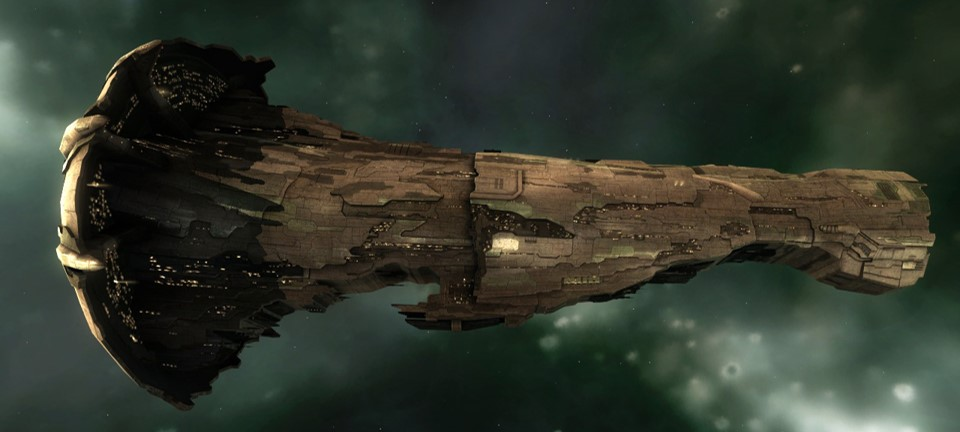
\includegraphics[width=3.5in]{avatarTitan.jpg}
    \caption{A mighty \textit{Avatar}-class Titan. \cite{avatar}}
    \label{fig:titan}
\end{figure}

\begin{equation} \label{eq:titanrecov}
\begin{aligned}
    \log_{10}{\widehat{R}} &= \mu + \sigma_{\textrm{supercap}} + 
    \rho_{\textrm{H-R00032}} + \beta_0 \log_{10} b_{\textrm{max}} \\
    &= 2.619576 + 6.837297 + 0.816951 + 0.011031 (1,836,944,290) \\
    &= 10.376016 \\
    & \\
    \Rightarrow \widehat{R} &= 10^{10.376016} \\
    &= 23,769,291,830 \textrm{ ISK}. \\
\end{aligned}
\end{equation}

Of course, this is incredibly lucrative for a single mission, but there are
virtually no players for whom this value is achievable. A more reasonable target
might be a medium noncombat ship; furthermore, we may readily suppose that the
aspiring pirate does not dare venture into Wormhole Space, preferring to remain
in safer, well-traveled Known Space regions. Selecting nevertheless the 
particularly lucrative region of Omist and a very large (albeit not maximal) 
bounty of 100,000,000 ISK should result in a hefty payoff, should the attack be
successful. An example of a medium noncombat ship is seen in \cref{fig:prowler}, 
and the predicted ISK recoverable is calculated in \cref{eq:medrecov}.

\begin{figure}[ht]
    \centering
    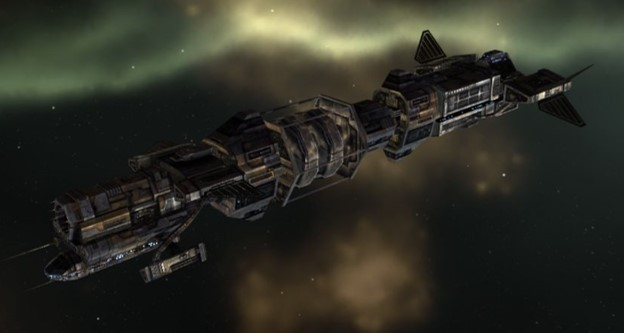
\includegraphics[width=3.5in]{prowlerBlockadeRunner.jpg}
    \caption{A \textit{Prowler}-class Blockade Runner, a medium noncombat ship.
    \cite{prowler}}
    \label{fig:prowler}
\end{figure}

\begin{equation} \label{eq:medrecov}
\begin{aligned}
    \log_{10}{\widehat{R}} &= \mu + \sigma_{\textrm{mednoncom}} + 
    \rho_{\textrm{Omist}} + \beta_0 \log_{10} b \\
    &= 2.619576 + 3.923020 + 0.694132 + 0.011031 \log_{10}(100,000,000) \\
    &= 7.324976 \\
    & \\
    \Rightarrow \widehat{R} &= 10^{7.324976} \\
    &= 21,133,722 \textrm{ ISK}.
\end{aligned}
\end{equation}

This predicted value is, of course, more than three orders of magnitude less than
the predicted ISK recoverable from destroying a Titan. However, there is still 
utility in maximizing the bounty and choosing a lucrative region. To show this, we
calculate in \cref{eq:cheapprowler} the predicted ISK recoverable for the same kind
of ship, but in the least valuable region and with no (logged) bounty.

\begin{equation} \label{eq:cheapprowler}
\begin{aligned}
    \log_{10}{\widehat{R}} &= \mu + \sigma_{\textrm{mednoncom}} \\
    &= 2.619576 + 3.923020 = 6.542596 \\
    & \\
    \Rightarrow \widehat{R} &= 10^{6.542596} = 3,488,156 \textrm{ ISK},
\end{aligned}
\end{equation}

a predicted return slightly less than one-sixth of the predicted ISK recoverable
for the medium noncombat ship with more valuable secondary factors chosen.

\section{Future directions}

With such a mass of data, it was inevitable that some valuable nuggets would be
trimmed out along with the necessary data processing. For instance, although we
observed a daily and five-hourly recurrence (seen in \cref{fig:acf}), we did not
treat the data differently depending on the time or date in which the ship was
destroyed. Future analysis could invoke tools from \textit{time series analysis},
elucidating these recurrent relationships. With more processing power or more time,
the amount of data could be increased from our meager three months; there are years
of Monthly Economic Reports available online. With enough time, it is possible that
we could even discern inflationary or deflationary patterns over time: the value of
ISK recoverable from a ship of a given kind or for a given region might 
systematically change over time.

Additionally, there are hundreds of megabytes of additional data in each MER that
we did not analyze; although these are purely economic data that do not directly
relate to the killdump, it is possible that they could shed light on parts of the
analysis that we did not fully interpret. For example, careful analysis of 
information like the destroyed value by region, seen below in \cref{fig:destroyed} 
--- or even the traffic report (\cref{fig:jumps}) --- could help us detect patterns
in the regions and better explain why some regions have larger ISK recoverable
coefficients $\rho_j$ compared to others.

\begin{figure}[ht]
    \centering
    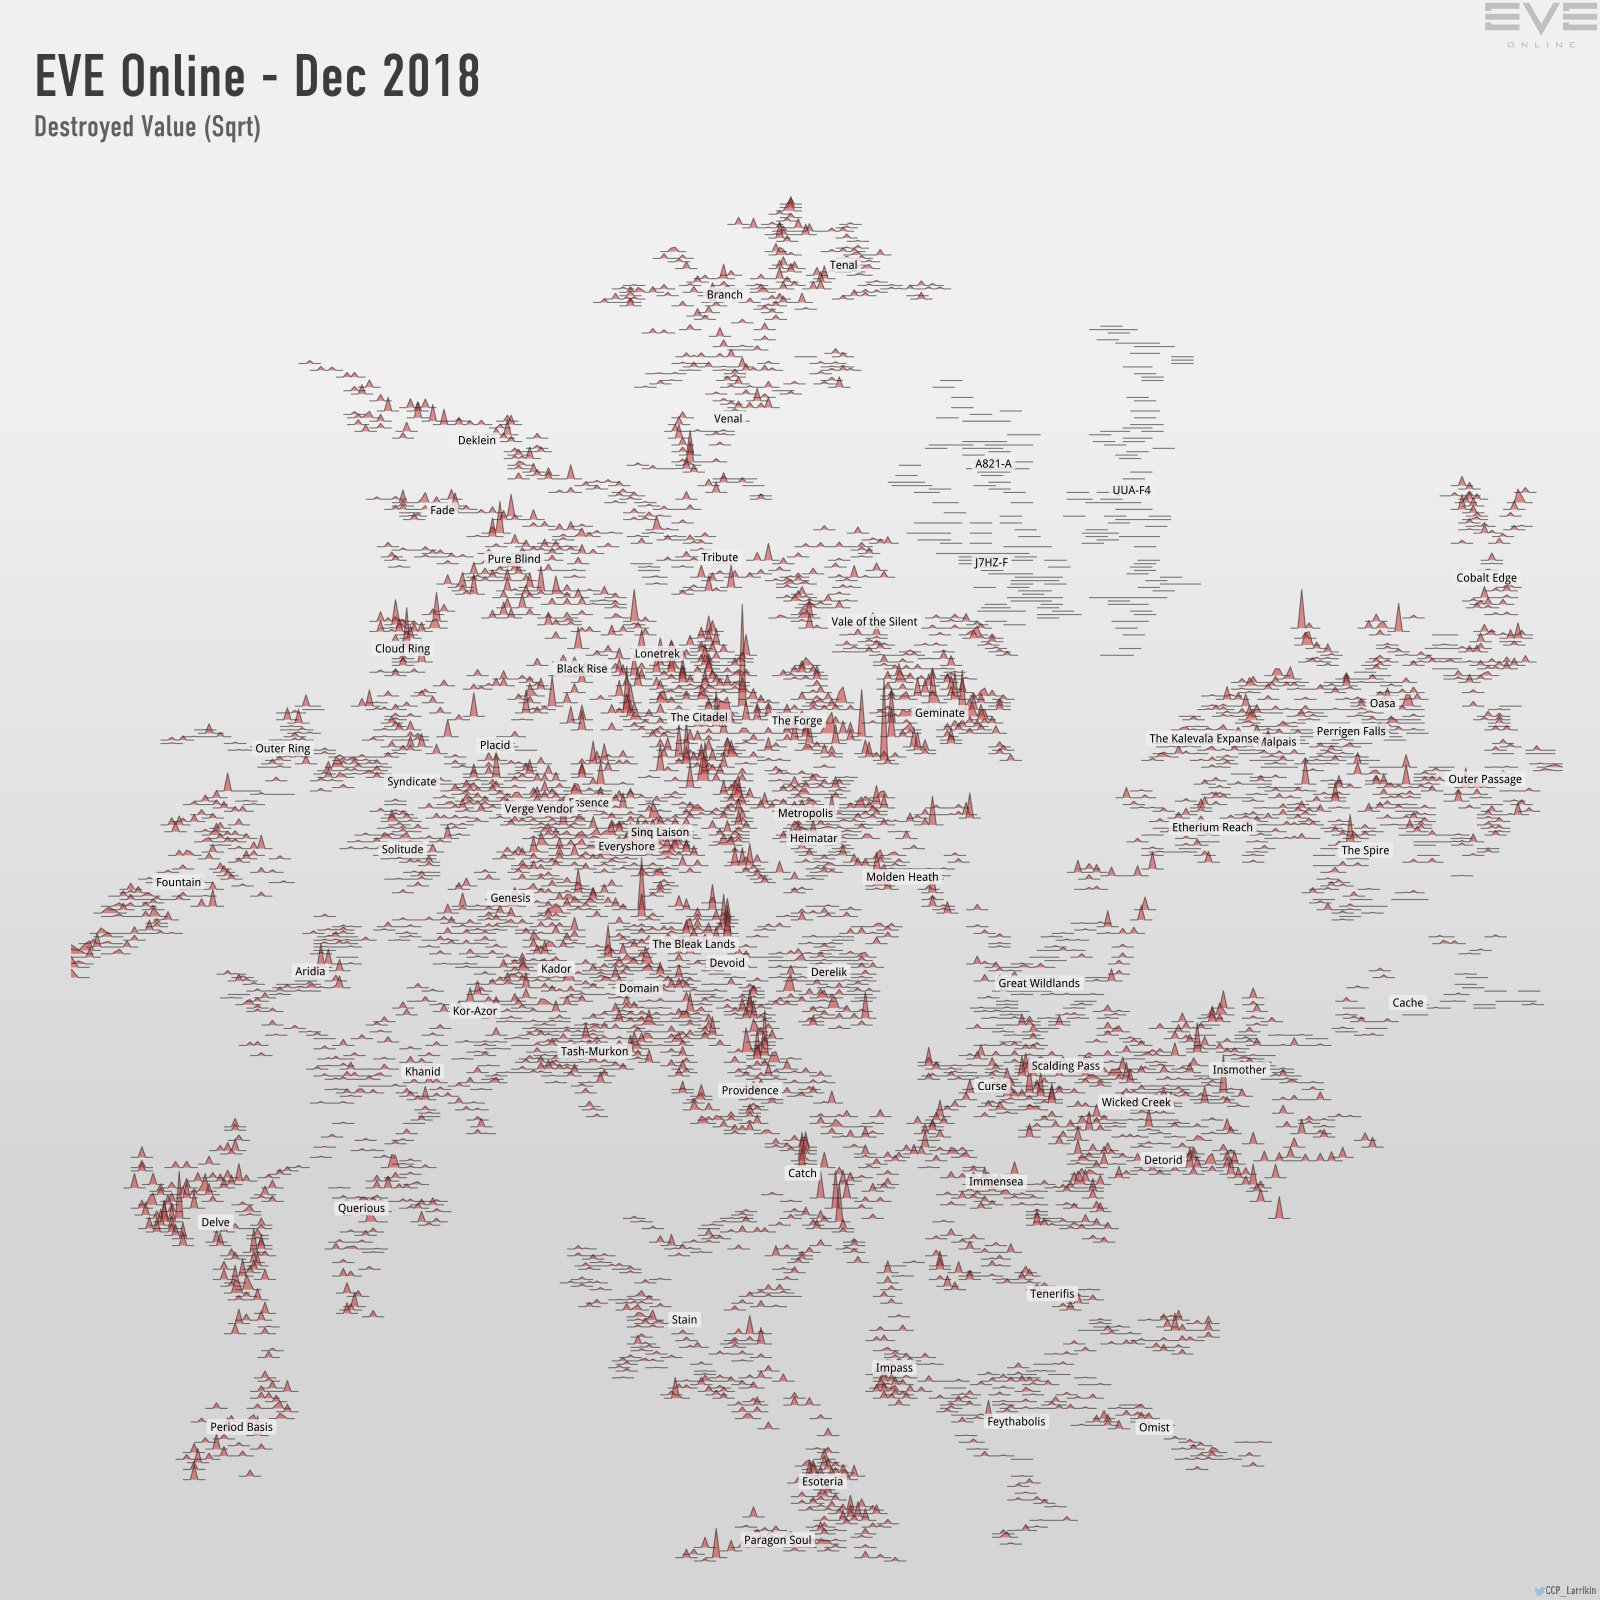
\includegraphics[width=3.5in]{destroyed_value_(sqrt).png}
    \caption{The square root of destroyed value by region in December 2018.
    \cite{MERdec2018}}
    \label{fig:destroyed}
\end{figure}

Finally, the spike in \cref{fig:loghist} of ships returning zero ISK recoverable (on
the log scale) suggest the use of a \textit{zero-inflated model}, which treats the
excess zeroes as distinct from the rest, which come from the typical normal
distribution. Such a model would be expected to improve our fit, and could possibly
elucidate why some ships have no recoverable ISK, while others have valuable salvage.

\section{Concluding remarks}

EVE Online is a game like no other. From its humble beginnings as an early-2000s
MMORPG from an unknown Icelandic developer to its current status as the undisputed
master canvas for human drama against a digital backdrop, New Eden has survived,
thrived, and evolved into something more intricate and more evocative than anyone
could have predicted at its initial release. Nowhere else can thousands of players
work together to decide the fate of a virtual star system, engage in intensive 
intergalactic politics, and navigate a complex economy, all without the risks that
come with such activities in the real world. Tens of thousands of players are made
happy by their time in New Eden, and I hope that this work, if nothing else, adds
a small drop of extra happiness for some few of them.

\backmatter
\newpage
\bibliographystyle{unsrt}
\bibliography{refs}

\newpage
\chapter[Appendix: Computer code]{Appendix: Computer code}
We include a Python script which, when the EVE data files are unzipped, collates
all the Killdump files into a specified directory, removes the logs concerning
only escape capsules (whose ISK recoverable value is always zero), and removes
unwanted columns from the data. This script is thus a major part of the
scalability of the project. \medskip

In addition, we include the R script with which all statistical analyses are
conducted. We used functions to perform further data cleanup, especially
summarizing across variables that were not found to be useful predictors in the
final model. Additionally, all plots were generated in this script. To that end,
the Tidyverse collection of packages was invaluable. \medskip

\section{Python code for data cleanup}

{\tiny
\begin{lstlisting}[language=Python]
###############################################################################
###                         Killdump-data-mover                             ###
###############################################################################
# Created by Jacob Williams for STAT 4870
# Built under Python 3.5
# Last modified: 2/13/2019

# A Python script for moving the Killdump.csv files from EVE Online's monthly
# economic report into the proper folder for analysis, as well as for modifying
# the files to remove unwanted data.

# Runs over each EVEOnline_MER_* directory (* a month and year); each directory
# contains one Killdump.csv. The script renames the file to YYYYMMMKilldump.csv
# where YYYY is the year and MMM is the month's abbreviation, and moves it to
# the killdumps directory.
# 
# It also deletes any row whose destroyedShipType is "Capsule" and deletes the
# columns whose entries are numeric for internal identification:
#   victimCorporationID             (the first column)
#   finalCorporationID              (the fourth column)
#   destroyedShipTypeID             (the seventh column)
#   solarSystemID                   (the eleventh column)
#   regionID                        (the thirteenth column)

import glob
import csv
import os
import re

basePath = os.path.dirname(os.path.realpath(__file__))

# Get the parent directory
def getParentDir(directory):
    return os.path.dirname(directory)

killDumpPath = basePath+"/killdumps"

for theDir in glob.iglob(basePath+'/EVEOnline_MER_*'):
    # Enter directory 
    os.chdir(theDir)
    parentDir = getParentDir(theDir)

    # Obtain the month and year from the current directory
    theYear = re.findall('\d+',theDir)[0]
    theMonth = (re.findall('[A-Z][a-z][a-z]\d',theDir)[0])[:-1]
        # some explanation: Finds capital letter followed by two lowercase
        # then a digit (to avoid 'Onl'); then deletes the digit
    
    # Rename and move the file
    for file in glob.glob('Killdump.csv'):
        os.rename(file,killDumpPath+'/'+theYear+theMonth+'Killdump.csv')

    # Return to main directory
    os.chdir(parentDir)

# Enter killdumps directory
os.chdir(killDumpPath)

# Perform data modification
for file in os.listdir(os.getcwd()):
    with open(file) as inp, open(file[:-4]+'_edited.csv','w') as out:
        writer = csv.writer(out)
        for r in csv.reader(inp):
            # Write only the desired rows and columns
            if r[8] != "Capsule":
                writer.writerow( (r[1],r[2],r[4],r[5],r[7],r[8],r[9],r[11],
                        r[13],r[14],r[15],r[16]) )

\end{lstlisting}
}
\section{R code for analysis}
{\tiny
\begin{lstlisting}[language=R]
###############################################################################
###                     EVE Online killdump analysis                        ###
###############################################################################

# Created by Jacob Williams for STAT 4870
# Built under R, version 3.5.3
# Last modified: 4/28/2019

###############################################################################
###                             Libraries                                   ###
###############################################################################
library(data.table)             # Fast data read-in
library(tidyverse)              # Fast data cleanup
library(car)                    # Model comparisons

###############################################################################
###                           ggplot2 parameters                            ###
###############################################################################

theme_update(text=element_text(size=20),
             axis.text.x=element_text(size=16),
             axis.text.y=element_text(size=16))


###############################################################################
###                             Read in data                                ###
###############################################################################

# Function by leerssej on StackOverflow:
#   https://stackoverflow.com/questions/11433432/
dat <- list.files(pattern = "*.csv") %>% 
  map_df(~fread(., stringsAsFactors = TRUE))


###############################################################################
###                             Clean data                                  ###
###############################################################################

# Set NA bounties to zero
dat$bountyClaimed[is.na(dat$bountyClaimed)] <- 0
sum(dat$bountyClaimed != 0)  # 54,265 nonzero bounties

# We remove fine-grained factors:
#   victimCorp
#   finalCorp
#   solarSystemName
#   destroyedShipType
dat$victimCorp <- NULL
dat$finalCorp <- NULL
dat$destroyedShipType <- NULL
dat$solarSystemName <- NULL

# Set factor variables to be factors (region is already)
dat$destroyedShipGroup <- as.factor(dat$destroyedShipGroup) # 89 levels
dat$victimAlliance <- as.factor(dat$victimAlliance)         # 1426 levels
dat$finalAlliance <- as.factor(dat$finalAlliance)           # 1021 levels

# Define response variable: recoverable ISK
dat$iskRecoverable <- dat$iskLost - dat$iskDestroyed

# Rename factors for convenience
colnames(dat)[colnames(dat)=="destroyedShipGroup"] <- "shipGroup"
colnames(dat)[colnames(dat)=="regionName"] <- "region"
colnames(dat)[colnames(dat)=="bountyClaimed"] <- "bounty"

# Fix the datetime variable, time only at the hour level
dat$date <- as.Date(dat$killTime)
dat$time <- format(as.POSIXct(dat$killTime),"%H:%M:%S")
dat$hour <- format(strptime(dat$time,"%H:%M:%S"),"%H") # get just hours
dat$hour <- as.factor(dat$hour)
dat$killTime <- NULL
dat$time <- NULL


###############################################################################
###                          Collapse data                                  ###
###############################################################################

# With well over 800,000 data points, collapsing is a good plan

# Reasonable factors to collapse: victimAlliance, shipGroup, region?
dat$regClaVal <- paste(dat$region,dat$shipGroup,dat$victimAlliance)
dat$regClaVal <- as.factor(dat$regClaVal) # 85,280 levels
dat$regClaVal <- NULL

# Could we add hour?
dat$regClaValHr <- paste(dat$region,dat$shipGroup,dat$victimAlliance,
                         dat$hour)
dat$regClaValHr <- as.factor(dat$regClaValHr) # 238,881 levels
dat$regClaValHr <- NULL

# There are too many levels with hour. Probably one of the other groups
#   would need to be cut out.

# Collapse the data by victimAlliance, shipGroup, region: 85,280 observations
byAGR <- dat %>% group_by(victimAlliance,shipGroup,region) %>%
  summarize(iskLost=mean(iskLost),iskDestroyed=mean(iskDestroyed),
            bounty=mean(bounty),iskRecoverable=mean(iskRecoverable))

# We wish to sort region and shipGroup by mean iskRecoverable


###############################################################################
###                       Initial modeling                                  ###
###############################################################################

  # Order regions from lowest to largest iskRecoverable
byAGR$region <- reorder(byAGR$region,byAGR$iskRecoverable)
lmReg <- lm(iskRecoverable~region,data=byAGR)
summary(lmReg)
# Not very significant results: only one p-value < 0.01, and it is 0.0077
  # E-R00026 (wormhole class 5) is the one W-space region that matters
  # Apparently lucrative regions: 
  #   Oasa, Derelik, Branch, Molden Heath, E-R00026
  #   Cobalt Edge, The Forge, ADR01, Tash-Murkon, Perrigen Falls,
  #   Wicked Creek, ADR03 (borderline), The Spire
# The R^2 value is only 0.000480, indicating very little variability in
#   iskRecoverable can be explained by the region.


# By shipGroup alone
byAGR$shipGroup <- reorder(byAGR$shipGroup,byAGR$iskRecoverable)
lmGro <- lm(iskRecoverable~shipGroup,data=byAGR) # cheapest: mining drone
summary(lmGro) # There are substantial differences here

# By bounty alone
lmBou <- lm(iskRecoverable~bounty,data=byAGR)
summary(lmBou)
  # There is a relationship, but is it this simple?

# We have reason to suppose that bounty is exponentially distributed:
hist(byAGR$bounty) # most bounties are zero
hist(byAGR$bounty[byAGR$bounty > 0])
hist(byAGR$bounty[byAGR$bounty > 1000000])
hist(byAGR$bounty[byAGR$bounty > 100000000]) # memorylessness property
hist(log10(byAGR$bounty[byAGR$bounty > 0])) # looks virtually normal

# Is there a logarithmic relationship between the log of bounty
#   and iskRecoverable?
byAGR$hasBounty <- 0
byAGR$hasBounty[byAGR$bounty > 0] <- 1
byAGR$hasBounty <- as.factor(byAGR$hasBounty)

byAGR$logBounty <- 0
byAGR$logBounty[byAGR$bounty > 0] <- log(byAGR$bounty[byAGR$bounty > 0])
lmLBo <- lm(iskRecoverable~hasBounty+logBounty,data=byAGR)
summary(lmLBo)

byHBo <- lm(iskRecoverable~hasBounty+bounty,data=byAGR)
summary(byHBo)
  # The variability explained by linear bounty is greater than logarithmic
  # but still small (R^2 < 0.01 in all cases)

# Predict by hour (with the full dataset)
lmFullHou <- lm(iskRecoverable~hour,data=dat)
summary(lmFullHou)
  # Only 04, 10, 11 are different from hour00
  # Probably not a useful predictor
rm(lmFullHou)

  # Too many rows in victimAlliance for direct lm
byAGR$victimAlliance <- reorder(byAGR$victimAlliance,byAGR$iskRecoverable)
allyISK <- group_by(byAGR,victimAlliance) %>% 
  summarize(iskRecoverable=mean(iskRecoverable))
hist(allyISK$iskRecoverable)
hist(allyISK$iskRecoverable[allyISK$iskRecoverable > 1000000])
hist(allyISK$iskRecoverable[allyISK$iskRecoverable > 100000000])
hist(allyISK$iskRecoverable[allyISK$iskRecoverable > 1000000000])
  # This appears to be exponential, too.
hist(log10(allyISK$iskRecoverable[allyISK$iskRecoverable > 0]))
  # Slightly right-skewed, perhaps, but much more reasonable again

# The format of the victim's alliances suggests a grouping
#   according to order of magnitude of mean iskRecoverable.

###############################################################################
###                   Continued data manipulation                           ###
###############################################################################

# We wish to combine into one group any ship with "mining" in its group name;
# likewise those with "electronic".
byAGR$shipGroup <- as.character(byAGR$shipGroup)

byAGR$isMining <- 0
byAGR$isMining[byAGR$shipGroup %like% "Mining"] <- 1

byAGR$isElectronic <- 0
byAGR$isElectronic[byAGR$shipGroup %like% "Electronic"] <- 1

byAGR$isMobile <- 0
byAGR$isMobile[byAGR$shipGroup %like% "Mobile"] <- 1

byAGR$shipGroup[byAGR$isMining==1] <- "Mining ship"
byAGR$shipGroup[byAGR$isElectronic==1] <- "Electronic ship"
byAGR$shipGroup[byAGR$isMobile==1] <- "Mobile ship"

byAGR$shipGroup <- as.factor(byAGR$shipGroup)

byAGR$isMining <- NULL
byAGR$isElectronic <- NULL
byAGR$isMobile <- NULL

# So we have reduced shipGroup to 75 factors, from 89; none were significantly
# different in iskRecoverable from the cheapest one.
# We need to reorder the group again.
byAGR$shipGroup <- reorder(byAGR$shipGroup,byAGR$iskRecoverable)
lmGroRed <- lm(iskRecoverable~shipGroup,data=byAGR)
summary(lmGroRed)


###############################################################################
###                         Logarithmic response                            ###
###############################################################################

# We seek to investigate whether we should work on orders of magnitude of
# iskRecoverable instead of the raw values. 

hist(byAGR$iskRecoverable)
hist(byAGR$iskRecoverable[byAGR$iskRecoverable > 1000])
hist(byAGR$iskRecoverable[byAGR$iskRecoverable > 100000])
hist(byAGR$iskRecoverable[byAGR$iskRecoverable > 10000000])
hist(log10(byAGR$iskRecoverable))

# Yes, we should. However, we have 4,702 zero values in byAGR, as well as some
# values in (0,1]. So we will log(iskRecoverable+1) for our models.
dat$logRecoverable <- log10(dat$iskRecoverable + 1)
byAGR$logRecoverable <- log10(byAGR$iskRecoverable + 1)

logReg <- lm(logRecoverable~region,data=byAGR)
summary(logReg) # This still does not appear useful!

logGro <- lm(logRecoverable~shipGroup,data=byAGR)
summary(logGro) # Virtually everything is incredibly significant!
  # We will still get a smaller number of shipGroups and work from thence

logBou <- lm(logRecoverable~bounty,data=byAGR)
summary(logBou) # R^2 = 0.002216, still pretty small

logLBo <- lm(logRecoverable~logBounty,data=byAGR)
summary(logLBo) # R^2 = 0.005346, but highly significant coefficients

logHou <- lm(logRecoverable~hour,data=dat)
summary(logHou)


###############################################################################
###                         Combine ship groups                             ###
###############################################################################

# We reassign the shipGroup variable to one with a smaller number of groups:
#   combatSmall: frigates, destroyers
#   combatMedium: cruisers, battlecruisers
#   combatLarge: battleships
#   combatCapital: carriers, dreadnoughts, force auxiliaries
#   combatSuperCapital: supercarriers and Titans
#   noncombatSmall: mining and expedition frigates, barges, exhumers
#   noncombatMedium: exhumers, industrials, blockade runners
#   noncombatLarge: command industrial ships
#   noncombatFreighter: freighters and jump freighters
#   noncombatCapital: capital industrial ships
#   starbase: Player-owned starbases and Upwell structures such as citadels

# Current levels of shipGroup (there are 89) and their reassignments
dat$shipKind[dat$shipGroup=="Assault Frigate"] <- "combatSmall"
dat$shipKind[dat$shipGroup=="Assembly Array"] <- "starbase"
dat$shipKind[dat$shipGroup=="Attack Battlecruiser"] <- "combatMedium"
dat$shipKind[dat$shipGroup=="Battleship"] <- "combatLarge"
dat$shipKind[dat$shipGroup=="Black Ops"] <- "combatLarge"
dat$shipKind[dat$shipGroup=="Blockade Runner"] <- "noncombatMedium"
dat$shipKind[dat$shipGroup=="Capital Industrial Ship"] <- "noncombatCapital"
dat$shipKind[dat$shipGroup=="Carrier"] <- "combatCapital"
dat$shipKind[dat$shipGroup=="Citadel"] <- "starbase"
dat$shipKind[dat$shipGroup=="Combat Battlecruiser"] <- "combatMedium"

dat$shipKind[dat$shipGroup=="Combat Recon Ship"] <- "combatMedium"  # Cruiser
dat$shipKind[dat$shipGroup=="Command Destroyer"] <- "combatSmall"
dat$shipKind[dat$shipGroup=="Command Ship"] <- "combatMedium" # battlecruiser
dat$shipKind[dat$shipGroup=="Compression Array"] <- "starbase"
dat$shipKind[dat$shipGroup=="Control Tower"] <- "starbase"
dat$shipKind[dat$shipGroup=="Corporate Hangar Array"] <- "starbase"
dat$shipKind[dat$shipGroup=="Corvette"] <- "combatSmall" #starter ship
dat$shipKind[dat$shipGroup=="Covert Ops"] <- "combatSmall" # frigate
dat$shipKind[dat$shipGroup=="Cruiser"] <- "combatMedium"
dat$shipKind[dat$shipGroup=="Cynosural Generator Array"] <- "starbase"

dat$shipKind[dat$shipGroup=="Cynosural System Jammer"] <- "starbase"
dat$shipKind[dat$shipGroup=="Deep Space Transport"] <- "noncombatMedium"
dat$shipKind[dat$shipGroup=="Destroyer"] <- "combatSmall"
dat$shipKind[dat$shipGroup=="Dreadnought"] <- "combatCapital"
dat$shipKind[dat$shipGroup=="Electronic Attack Ship"] <- "combatSmall"
dat$shipKind[dat$shipGroup=="Electronic Warfare Battery"] <- "starbase"
dat$shipKind[dat$shipGroup=="Encounter Surveillance System"] <- "starbase"
dat$shipKind[dat$shipGroup=="Energy Neutralizing Battery"] <- "starbase"
dat$shipKind[dat$shipGroup=="Engineering Complex"] <- "starbase"
dat$shipKind[dat$shipGroup=="Exhumer"] <- "noncombatLarge"

dat$shipKind[dat$shipGroup=="Expedition Frigate"] <- "noncombatSmall"
dat$shipKind[dat$shipGroup=="Flag Cruiser"] <- "combatMedium"
dat$shipKind[dat$shipGroup=="Force Auxiliary"] <- "combatCapital"
dat$shipKind[dat$shipGroup=="Force Recon Ship"] <- "combatMedium" # cruiser
dat$shipKind[dat$shipGroup=="Forward Operating Base"] <- "starbase"
dat$shipKind[dat$shipGroup=="Freighter"] <- "noncombatFreighter"
dat$shipKind[dat$shipGroup=="Frigate"] <- "combatSmall"
dat$shipKind[dat$shipGroup=="Heavy Assault Cruiser"] <- "combatMedium"
dat$shipKind[dat$shipGroup=="Heavy Fighter"] <- "combatSmall" # drone
dat$shipKind[dat$shipGroup=="Heavy Interdiction Cruiser"] <- "combatMedium"

dat$shipKind[dat$shipGroup=="Industrial"] <- "noncombatMedium"
dat$shipKind[dat$shipGroup=="Industrial Command Ship"] <- "noncombatLarge"
dat$shipKind[dat$shipGroup=="Interceptor"] <- "combatSmall" # frigate
dat$shipKind[dat$shipGroup=="Interdictor"] <- "combatSmall" # destroyer
dat$shipKind[dat$shipGroup=="Jump Freighter"] <- "noncombatFreighter"
dat$shipKind[dat$shipGroup=="Jump Portal Array"] <- "starbase"
dat$shipKind[dat$shipGroup=="Laboratory"] <- "starbase"
dat$shipKind[dat$shipGroup=="Light Fighter"] <- "combatSmall" # drone
dat$shipKind[dat$shipGroup=="Logistics"] <- "combatSmall" # cruiser
dat$shipKind[dat$shipGroup=="Logistics Frigate"] <- "combatSmall" 

dat$shipKind[dat$shipGroup=="Marauder"] <- "combatLarge" # battleship
dat$shipKind[dat$shipGroup=="Mining Barge"] <- "noncombatMedium"
dat$shipKind[dat$shipGroup=="Mining Drone"] <- "noncombatSmall"
dat$shipKind[dat$shipGroup=="Mobile Cyno Inhibitor"] <- "starbase"
dat$shipKind[dat$shipGroup=="Mobile Depot"] <- "starbase"
dat$shipKind[dat$shipGroup=="Mobile Hybrid Sentry"] <- "starbase"
dat$shipKind[dat$shipGroup=="Mobile Laser Sentry"] <- "starbase"
dat$shipKind[dat$shipGroup=="Mobile Micro Jump Unit"] <- "starbase"
dat$shipKind[dat$shipGroup=="Mobile Missile Sentry"] <- "starbase"
dat$shipKind[dat$shipGroup=="Mobile Projectile Sentry"] <- "starbase"

dat$shipKind[dat$shipGroup=="Mobile Reactor"] <- "starbase"
dat$shipKind[dat$shipGroup=="Mobile Scan Inhibitor"] <- "starbase"
dat$shipKind[dat$shipGroup=="Mobile Siphon Unit"] <- "starbase"
dat$shipKind[dat$shipGroup=="Mobile Tractor Unit"] <- "starbase"
dat$shipKind[dat$shipGroup=="Mobile Warp Disruptor"] <- "starbase"
dat$shipKind[dat$shipGroup=="Moon Mining"] <- "starbase"
dat$shipKind[dat$shipGroup=="Orbital Construction Platform"] <- "starbase"
dat$shipKind[dat$shipGroup=="Orbital Infrastructure"] <- "starbase"
dat$shipKind[dat$shipGroup=="Personal Hangar"] <- "starbase"
dat$shipKind[dat$shipGroup=="Prototype Exploration Ship"] <- "combatSmall" 

dat$shipKind[dat$shipGroup=="Refinery"] <- "starbase"
dat$shipKind[dat$shipGroup=="Reprocessing Array"] <- "starbase"
dat$shipKind[dat$shipGroup=="Scanner Array"] <- "starbase"
dat$shipKind[dat$shipGroup=="Sensor Dampening Battery"] <- "starbase"
dat$shipKind[dat$shipGroup=="Shield Hardening Array"] <- "starbase"
dat$shipKind[dat$shipGroup=="Ship Maintenance Array"] <- "starbase"
dat$shipKind[dat$shipGroup=="Shuttle"] <- "noncombatSmall"
dat$shipKind[dat$shipGroup=="Silo"] <- "starbase"
dat$shipKind[dat$shipGroup=="Stasis Webification Battery"] <- "starbase"
dat$shipKind[dat$shipGroup=="Stealth Bomber"] <- "combatSmall"

dat$shipKind[dat$shipGroup=="Strategic Cruiser"] <- "combatMedium"
dat$shipKind[dat$shipGroup=="Supercarrier"] <- "combatSuperCapital"
dat$shipKind[dat$shipGroup=="Support Fighter"] <- "combatSmall"
dat$shipKind[dat$shipGroup=="Tactical Destroyer"] <- "combatSmall"
dat$shipKind[dat$shipGroup=="Titan"] <- "combatSmall"
dat$shipKind[dat$shipGroup=="Upwell Cyno Beacon"] <- "starbase"
dat$shipKind[dat$shipGroup=="Upwell Cyno Jammer"] <- "starbase"
dat$shipKind[dat$shipGroup=="Upwell Jump Gate"] <- "starbase"
dat$shipKind[dat$shipGroup=="Warp Scrambling Battery"] <- "starbase"

dat$shipKind <- as.factor(dat$shipKind)
levels(dat$shipKind) # looks as we would like

###############################################################################
###                         Logarithmic bounty                              ###
###############################################################################

# Given our histograms, we wish bounty to operate on a logarithmic scale also
# There are lots of zero bounties, as well as bounties less than 1
sum(dat$bounty == 0)
sum((dat$bounty != 0 & dat$bounty < 1)) # 203 nonzero bounties less than 1

# Because we are concerned with order of magnitude, it's not a big deal to
#   treat these bounties as zero. So we can log10(bounty + 1) as we did with
#   iskRecoverable!
dat$logBounty <- 0
dat$logBounty[dat$bounty > 0] <- log10(dat$bounty[dat$bounty > 0] + 1)

###############################################################################
###                           Regroup the data                              ###
###############################################################################

# We have found that:
#   region is not a good predictor
#   hour is not a good predictor
#   victimAlliance and finalAlliance have too many levels
#     and too much political complexity to group tighter
#   shipGroup, or at least shipKind, is a good predictor
#   bounty is as well (we log it)

# We will create a new condensed dataset accounting for this.
byAARK <- dat %>% group_by(victimAlliance,finalAlliance,region,shipKind) %>% 
  summarize(logRecoverable=mean(logRecoverable),logBounty=mean(logBounty))
  # We can customize the collapsed variables to control the size of the data

byAARK$victimAlliance <- NULL
byAARK$finalAlliance <- NULL

###############################################################################
###                 Analysis with the new dataset                           ###
###############################################################################

# We conduct a linear model of the logarithm of ISK recoverable against the 
# shipKind and the logarithm of the bounty, allowing for interactions between
# them.
byAARK$shipKind <- reorder(byAARK$shipKind,byAARK$logRecoverable)

logKi <- lm(logRecoverable~shipKind,data=byAARK)
summary(logKi)
confint(logKi)

logKiBo <- lm(logRecoverable~shipKind*logBounty,data=byAARK)
summary(logKiBo)
  # Most interactions, except between bounty and small ships, are not sig.

# Without interactions:
logKB <- lm(logRecoverable~shipKind+logBounty,data=byAARK)
summary(logKB)
  # Very little difference in R^2 or residual SE! And now bounty is sig.

byAARK$region <- reorder(byAARK$region,byAARK$logRecoverable)
logReg2 <- lm(logRecoverable~region,data=byAARK)
summary(logReg2)
  # On the logarithmic scale, this becomes significant...

lmReg2 <- lm(I(exp(logRecoverable)-1)~region,data=byAARK)
summary(lmReg2)
  # The ordering isn't necessarily on point, but there is significance heres

### Let's create a model involving region, shipKind, and bounty
logKiBoRe <- lm(logRecoverable~shipKind*logBounty+region*logBounty,data=byAARK)
summary(logKiBoRe)

# Bounty matters for little ships only, but we don't want to drag others in


### Without interactions
byAARK$shipKind <- reorder(byAARK$shipKind,byAARK$logRecoverable)
logKBR <- lm(logRecoverable~shipKind+region+logBounty,data=byAARK)
summary(logKBR)
plot(logKBR)

###############################################################################
###                 A further analysis of time of day                       ###
###############################################################################

# We can manage the amount of data that we have, and suspect that on the
#   logarithmic scale the hour of day, or perhaps the date, will be important.
byHour <- dat %>% group_by(hour) %>% 
  summarize(logRecoverable=mean(logRecoverable))

plot(logRecoverable~hour,data=byHour)
  # See, now, this looks like something important

# With error bars, though, perhaps not
byHAARK <- dat %>% group_by(hour,shipKind,region,victimAlliance,
                            finalAlliance) %>%
  summarize(logRecoverable=mean(logRecoverable),logBounty=mean(logBounty))

plot(logRecoverable~hour,data=byHAARK) # It's much less clear now

logHour <- lm(logRecoverable~hour,data=byHAARK)
summary(logHour)
  # We see differences!

# It is not entirely clear how these should be ordered, to my mind,
# although hours 12-23 seem to be grouped somewhat. Maybe a sinusoid?
byHAARK$hour <- reorder(byHAARK$hour,byHAARK$logRecoverable)
logHouOrd <- lm(logRecoverable~hour,data=byHAARK)
summary(logHouOrd)

# Let's plot a time series with date and hour
byHoDa <- dat %>% group_by(date,hour) %>%
  summarize(logRecoverable=mean(logRecoverable))

ggplot(aes(x=date,y=logRecoverable),data=byHoDa) + geom_point()
ggplot(aes(x=hour,y=logRecoverable),data=byHoDa) + geom_point()
  # I think the difference is more obvious in the date plot

logDate <- lm(logRecoverable~date,data=byHoDa)
summary(logDate)
  # In the linear model context, the date doesn't matter

hourACF <- acf(byHoDa$logRecoverable,xlab="Lag (hours)",ylab="Autocorrelation",
    main="Autocorrelation of recoverable ISK by hour")
# We see autocorrelation peaking at period 23-24!
  # And 1, but this is perhaps to be expected

# Can we find this just grouping by date?
byDate <- dat %>% group_by(date,victimAlliance) %>% 
  summarize(logRecoverable=mean(logRecoverable))

acf(byDate$logRecoverable) # Not a whole lot going on here!


###############################################################################
###                           The final model                               ###
###############################################################################

### We found that shipKind is the major predictor, but that region and
###   logBounty matter as well. In addition, when the ship is of a small kind,
###   there is an interaction between shipKind and logBounty.
### The response is logRecoverable.

# An indicator variable for small ships
byAARK$smallCombat <- 0
byAARK$smallCombat[byAARK$shipKind=="combatSmall"] <- 1
byAARK$smallNonCombat <- 0
byAARK$smallNonCombat[byAARK$shipKind=="noncombatSmall"] <- 1

byAARK$shipKind <- reorder(byAARK$shipKind,byAARK$logRecoverable)
byAARK$region <- reorder(byAARK$region,byAARK$logRecoverable)
fit <- lm(logRecoverable~shipKind+logBounty+region+
            logBounty:smallCombat+logBounty:smallNonCombat,data=byAARK)
summary(fit)
plot(fit)


###############################################################################
###                     Graphics and interpretations                        ###
###############################################################################

# Do we need different indicators for small combat and small noncombat ships?
linearHypothesis(fit,"logBounty:smallCombat = logBounty:smallNonCombat") # yes

# The autocorrelation in hours is interesting, but it is a very subtle 
# distinction, so we will relegate its analysis to future work
acf(byHoDa$logRecoverable,xlab="Lag (hours)",ylab="Autocorrelation",
               main="Autocorrelation of recoverable ISK by hour")


# Prediction graph for logBounty.
#   For our prediction, we will use combatMedium and The Citadel as "average"
#   shipKind and region, respectively.
predNotSmall <- tibble(
  logBounty=seq(min(byAARK$logBounty),max(byAARK$logBounty),length=5000),
  smallCombat=rep(0,5000),
  smallNonCombat=rep(0,5000),
  region=rep("The Citadel",5000),
  shipKind=rep("combatMedium",5000)
)
predNotSmall$logRecoverable <- predict(fit,newdata=predNotSmall)

predSmallCombat <- tibble(
  logBounty=seq(min(byAARK$logBounty),max(byAARK$logBounty),length=5000),
  smallCombat=rep(1,5000),
  smallNonCombat=rep(0,5000),
  region=rep("The Citadel",5000),
  shipKind=rep("combatSmall",5000)
)
predSmallCombat$logRecoverable <- predict(fit,newdata=predSmallCombat)

predSmallNonCombat <- tibble(
  logBounty=seq(min(byAARK$logBounty),max(byAARK$logBounty),length=5000),
  smallCombat=rep(0,5000),
  smallNonCombat=rep(1,5000),
  region=rep("The Citadel",5000),
  shipKind=rep("noncombatSmall",5000)
)
predSmallNonCombat$logRecoverable <- predict(fit,newdata=predSmallNonCombat)

byAARK$colorVar <- "Large ship"
byAARK$colorVar[byAARK$smallCombat==1] <- "Small combat ship"
byAARK$colorVar[byAARK$smallNonCombat==1] <- "Small noncombat ship"

ggplot(byAARK,aes(logBounty,logRecoverable)) + 
  geom_point(aes(color=colorVar),show.legend=TRUE) + 
  geom_line(data=predNotSmall,color="green",size=2) + 
  geom_line(data=predSmallCombat,color="red",size=2) + 
  geom_line(data=predSmallNonCombat,color="blue",size=2) + 
  theme(legend.title = element_blank()) +
  xlab("Logarithm of bounty") + ylab("Logarithm of recoverable ISK") + 
  scale_color_manual(values=c("#00BA38","#F8766D","#00BFC4"))

# Histograms for the recoverable ISK and its logarithm
byAARK$iskRecoverable <- 10^(byAARK$logRecoverable) + 1

ggplot(byAARK,aes(iskRecoverable)) + 
  geom_histogram(bins=50,color="red") + 
  xlab("Recoverable ISK") + ylab("Count")

ggplot(byAARK,aes(logRecoverable)) + 
  geom_histogram(bins=50,color="blue") + 
  xlab("Logarithm of recoverable ISK") + ylab("Count")

# Boxplot for the shipKind effect
ggplot(byAARK,aes(shipKind,logRecoverable)) + 
  geom_boxplot() + 
  theme(axis.text.x=element_text(angle=90,vjust=-0.5)) +
  xlab("") + ylab("Logarithm of recoverable ISK")

\end{lstlisting}
}

\newpage
\thispagestyle{empty}
\mbox{}
\newpage

\end{document}
